\startchapter{Systematic Uncertainties}
\label{chapter:systematics}

In order to properly assess the significance of any discrepancies between predicted yields of signal and SM background and of the observed collision data, it is important to assign uncertainties to all sources which may limit the precision and accuracy of yield predictions. In addition to a limited precision arising from statistical uncertainty\footnote{See Chapter \ref{sec:mc_intro} for a discussion of the origin of statistical uncertainty in MC simulations.}, there may be inaccuracies in the values of various parameters input to the simulation due to a limited precision with which their values are known. These inaccuracies can systematically shift predicted production rates and kinematic properties of the simulated processes. Systematic uncertainties aim to quantify the uncertainty of  predicted yields of signal and SM background processes within each region and bin\footnote{See Section \ref{sec:binning_strategy} for details of the binning in \minms performed in the SR} used in the search that could result from each source of potential inaccuracy in the modelling. 

Systematic uncertainties (or simply ``systematics") are broadly classified into two categories according to their origin: theoretical and experimental. Theoretical systematics account for inaccuracies that could result from a limited knowledge of parameters involved in modelling the production and decay mechanisms resulting from \(pp\) collision events at the LHC. Experimental systematics are evaluated to account for the limited accuracy and precision involved with the highly detailed model used to simulate the operation of the ATLAS detector. In addition to the limited precision of the measured LHC beam luminosity, uncertainties arise from a wide range of sources involved with simulating the detection and reconstruction of collision events. These include limitations associated with the Geant4 model \cite{Geant4} used to simulate the passage of particles through the detector, with modelling the data acquisition and readout systems employed by each sub-detector\footnote{See Section \ref{sec:ATLAS_detector_intro} for a description of the ATLAS sub-detectors.}, and with simulating the reconstruction and identification of physics objects\footnote{See Section \ref{sec:object_defs} for a presentation of the reconstructed physics objects used in this search.} using the simulated readouts from all the sub-detectors. Additional uncertainties arise from time-dependent modifications to the simulation, such as the reweighting of simulated events to account for time-varying pileup\footnote{See Section \ref{sec:evt_wts} for a discussion of the pileup reweighting weight used to account for time-varying pileup conditions in the detector.} conditions in the detector.

Experimental systematics are generally constrained in the process of calibrating particular physics objects reconstructed in the ATLAS detector using the ATLAS collision data, and as a result are generally considered quite well-defined and robust. In contrast, the choice of uncertainty to assign to theoretical parameters can be much less clear, as constraints from experimental results may be sparse, or in some cases such as appropriate choice of renormalization scale in perturbative QCD calculations \cite{PDG_2018}, essentially non-existent. 

Experimental and theoretical systematic uncertainties are evaluated in all analysis regions and bins for the SM background processes. Due to the negligible yield of the DH signal process in the CRs, systematic uncertainties are only evaluated for the signal process in the SRs.

\section{Experimental Systematics}

Experimental systematics are evaluated for all physics objects considered in the search, and for the LHC beam luminosity. 

The integrated luminosity \(\mathcal{L}_\text{int}\) recorded by the ATLAS detector for the full data set considered in this search is known with a precision of \(1.7\%\) \cite{ATLAS-CONF-2019-021}. Since, from Eq. \ref{eq:integrated_lumi}, the total number of recorded collision events scales linearly with the integrated beam luminosity, propagating this \(\pm1.7\%\) systematic to the yields results in coherent \(1.7\%\) up and down shifts of the predicted yield for each process across all analysis regions and bins.

For a given systematic uncertainty on a parameter \(k\) used in the reconstruction of physics objects, the general procedure for propagating the systematic uncertainty to the predicted yield \(N_p\) of a process \(p\) in a bin \(j\) is as follows:

\begin{itemize}
\item Repeat the reconstruction with \(k\) shifted up by one standard deviation: \(k\text{ up} = k+\sigma_k\).
\item Evaluate the predicted yield in the bin \(N_\text{\(p\), \(k\) up, bin \(j\)}\) with updated simulation. The ``up" systematic yield uncertainty is:
\begin{equation}
\label{eq:exp_systs}
\text{syst}\text{(exp, \(p\), \(k\) up, bin \(j)\)} = N_\text{\(p\), \(k\) up, \(j\)} - N_\text{\(p\), nom, \(j\)}
\end{equation}
\noindent where \(N_\text{\(p\), nom, \(j\)}\) is the nominal yield.
\item Repeat the above process with \(k\) shifted down by one standard deviation to evaluate the ``down" systematic uncertainty.
\end{itemize}

\noindent Due to statistical uncertainties arising from the limited number of MC events available to evaluate shifted yields, asymmetries between the up and down yield shifts in the above procedure can occur simply due to statistical fluctuations in the number of events which fall into each bin, rather than from actual asymmetries in the underlying distribution being sampled. For this reason, the propagated yield systematics are symmetrized in each bin as follows:

\begin{equation}
\label{eq:exp_systs_symm}
\text{syst}\text{(exp, \(p\), \(k\) symm, bin \(j\))}= \pm\Bigg(\frac{N_\text{\(p\), \(k\), up, \(j\)} - N_\text{\(p\), \(k\), down, \(j\)}}{2}\Bigg)
\end{equation}

Table \ref{tab:exp_systs} summarizes the sources of experimental systematics considered for all physics objects in the search. 

\begin{table}
\centering
\caption{Sources of experimental systematic uncertainty considered for all physics objects used in the search. }
\label{tab:exp_systs}
\footnotesize{
\begin{tabular}{l p{11cm}}
\toprule
\textbf{Physics Object} & \textbf{Systematic Uncertainties Considered} \\
\midrule
\midrule
Electrons & \(-\) Reconstruction, ID and isolation efficiency \newline \(-\) Energy scale and resolution \\
\midrule
Muons & \(-\) Reconstruction, ID and isolation efficiency \newline \(-\) Trigger efficiency \newline \(-\) Energy scale and resolution \newline \(-\) Track-to-vertex association \\
\midrule
\(R=0.4\) Jets & \(-\) Energy scale and resolution \newline \(-\) Quark flavour composition \newline \(-\) Jet-vertex association \newline \(-\) Pileup \newline \(-\) \btag efficiency \\
\midrule
TAR jets & \(-\) \(R=0.2\) subjets input to TAR algo \newline \phantom{xl} (consider same sources as for \(R=0.4\) jets) \newline \(-\) Uncertainties associated with tracks input to TAR algo \\
\midrule
\met & \(-\) Soft terms used in \met calculation \newline \phantom{xl} (note that uncertainties associated with other objects used in the \phantom{xxl}\met calculation are propagated to \met, so are not classified as \phantom{xxl}\met systematics) \\
\bottomrule
\end{tabular}}
\end{table}

Figure \ref{fig:exp_syst_shifts_bkg} shows the envelope of all symmetrized shifts in the total predicted yield of all SM backgrounds in the SRs due to the sources of experimental systematics considered for each type of physics object. Figure \ref{fig:exp_syst_shifts_sig} shows the same set of envelopes for a sample signal point at \((\ms, \mZp)=(210, 2100)~\GeV\). Comparing the yield shifts associated with the reconstruction of the various physics objects, the experimental systematics are dominated by sources of uncertainty associated with the reconstruction of \(R=0.4\) jets and \(R=0.2\) TAR subjets in the merged SR. The \(R=0.2\) TAR subjets uncertainties produce relatively small yield shifts in the resolved SR because TAR jets are not used in this region. Shifts in predicted yield are also notably smaller for the signal model compared with the SM background processes. 
%This is likely due to the larger number of MC simulated events which are admitted into the SRs for the signal process, and the consequently smaller relative statistical fluctuations in yield shifts due to varying sources of uncertainty in the object reconstruction.

\begin{figure}[htbp]
  \centering
    \begin{subfigure}[t]{0.48\textwidth}
    \centering
     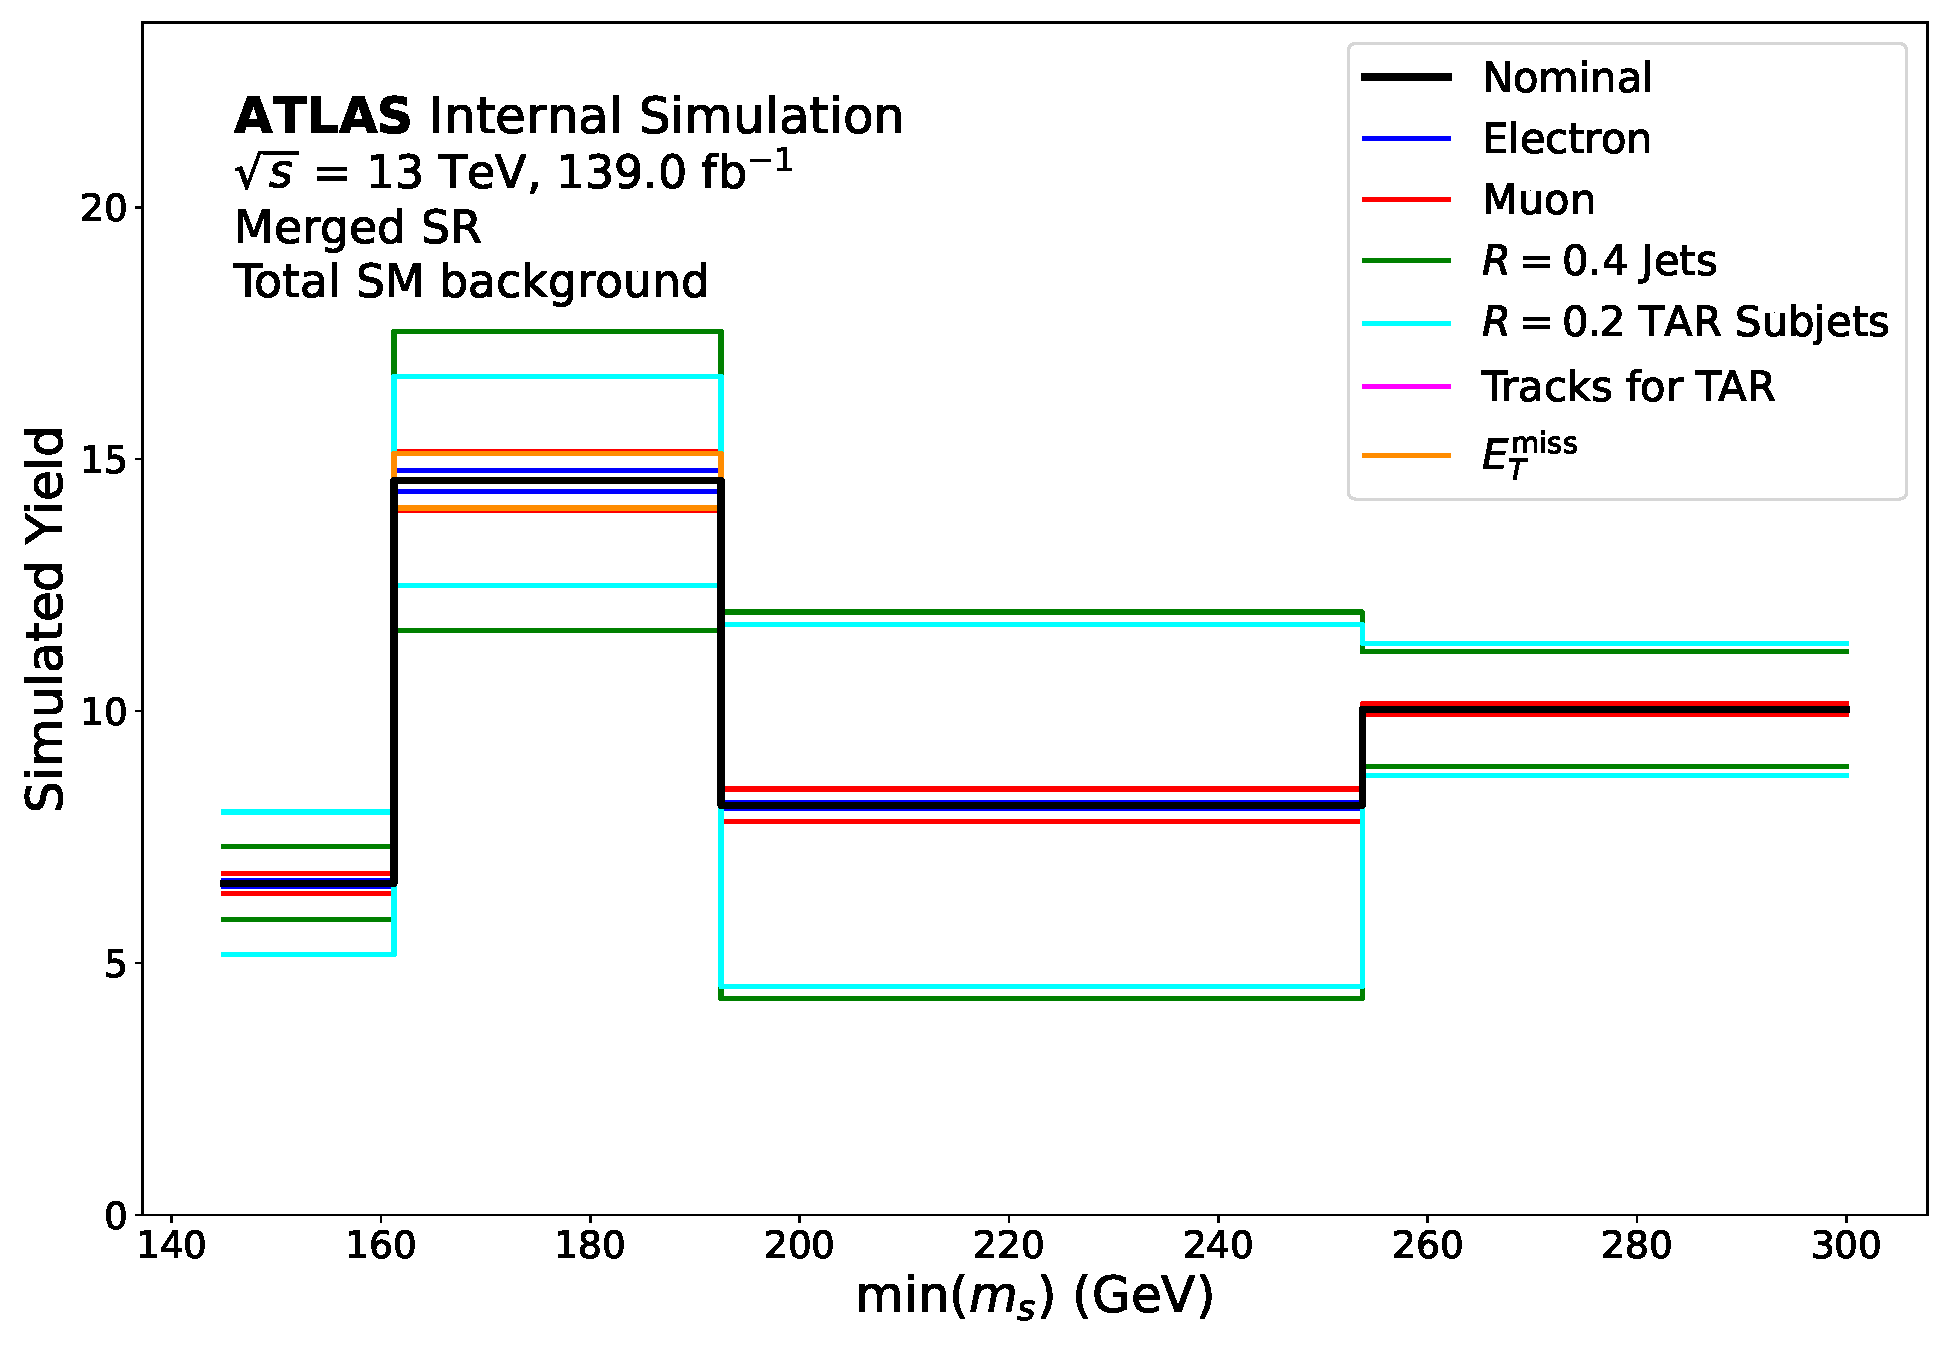
\includegraphics[width = 0.99\textwidth]{Figures/6/exp_systs_total_bkg_SR_mgd_TARJets10_minmS_mgd.pdf}
    \caption{Merged SR}
    \end{subfigure}
    \begin{subfigure}[t]{0.48\textwidth}
    \centering
     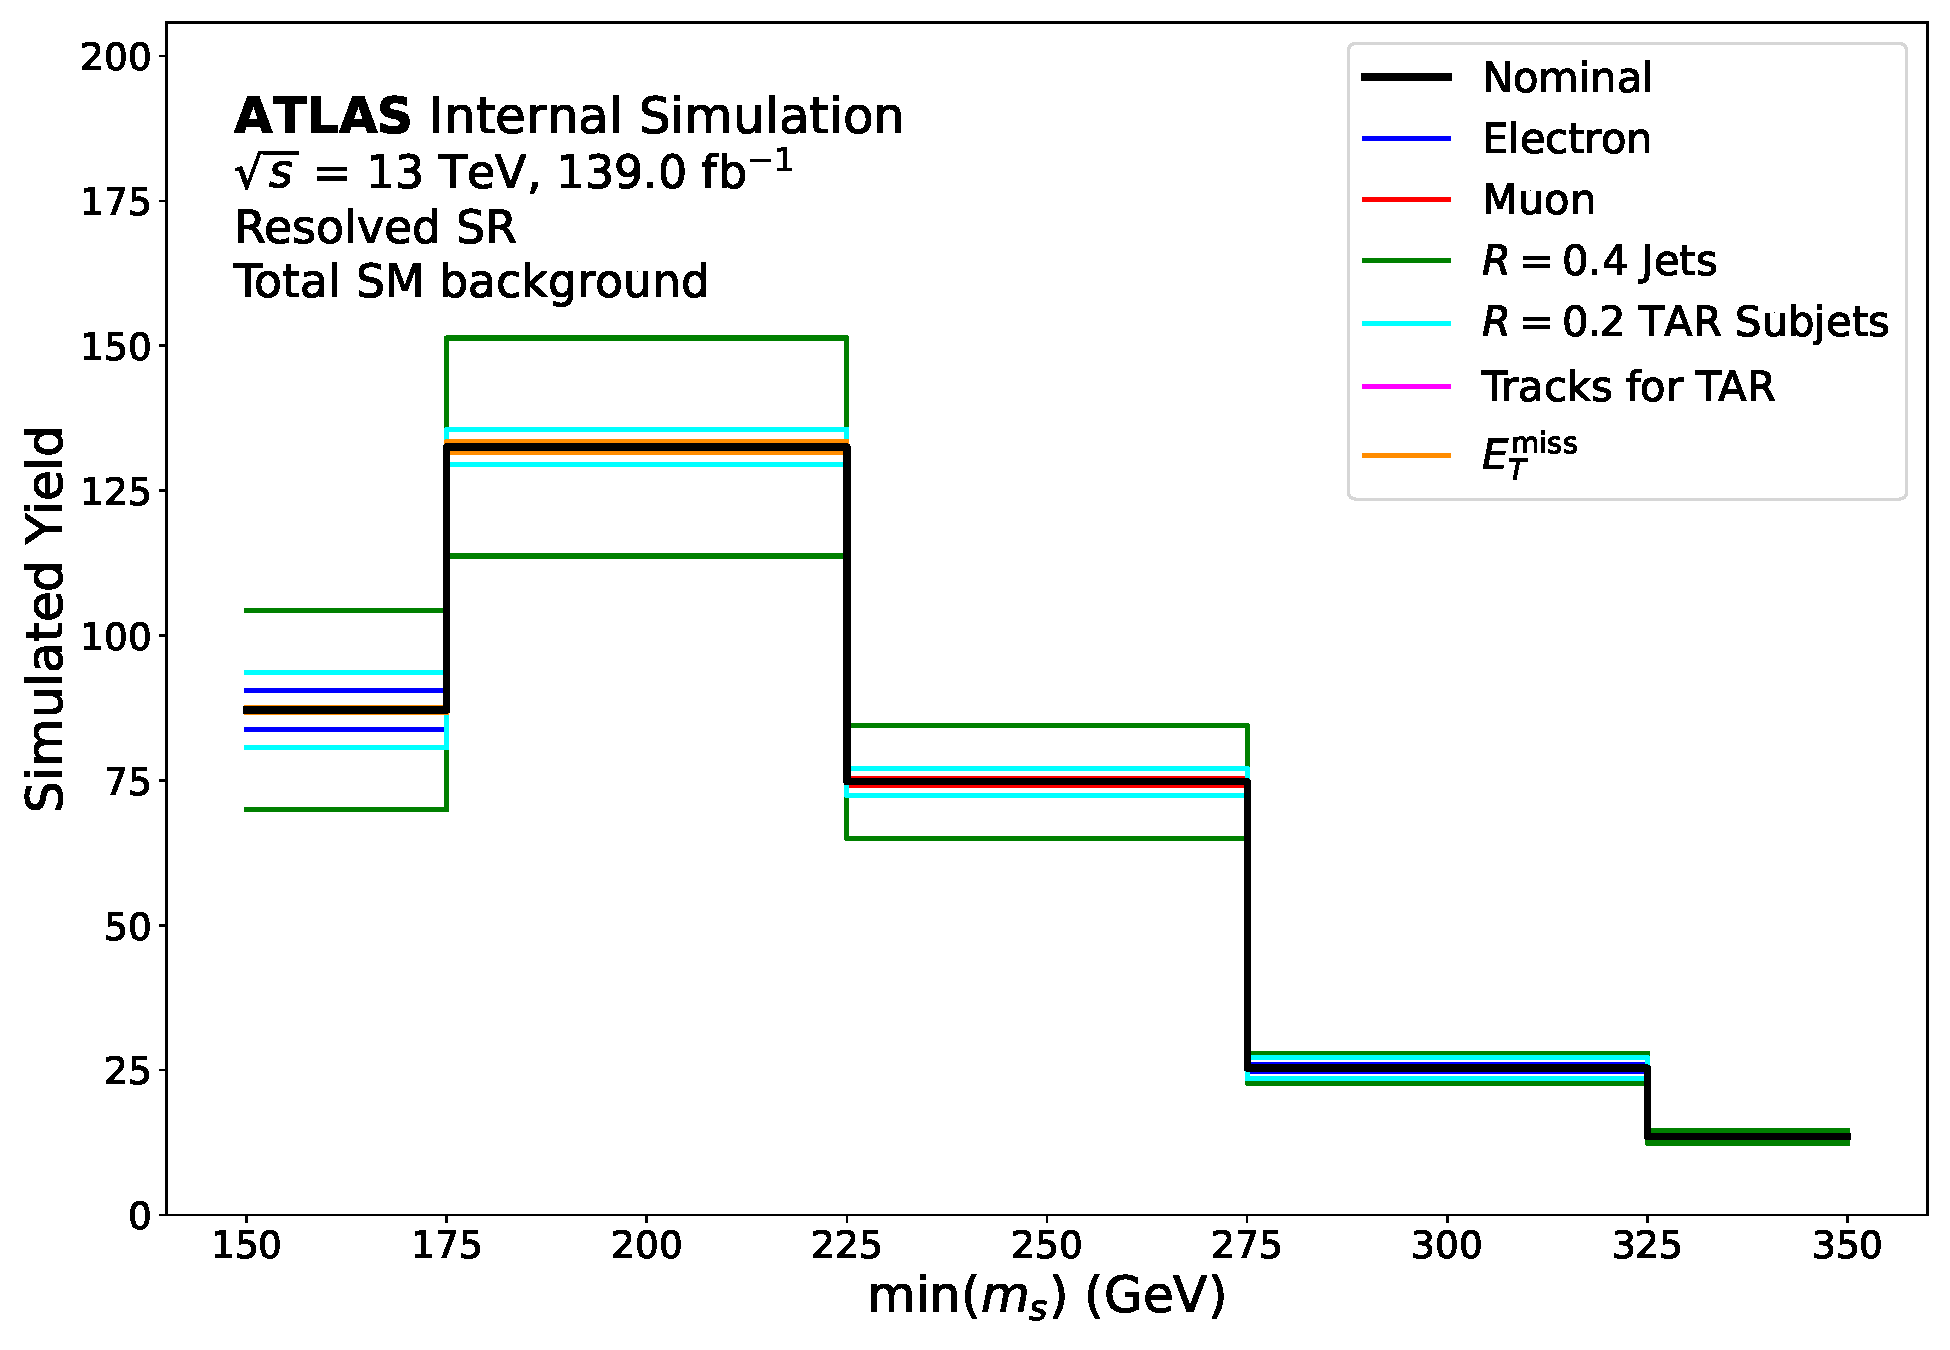
\includegraphics[width = 0.99\textwidth]{Figures/6/exp_systs_total_bkg_SR_res_TARJets10_minmS_res.pdf}
     \caption{Resolved SR}
    \end{subfigure}
    \caption{Envelope of shifts in the total predicted yield of SM background processes in the merged (left) and resolved (right) SRs due to experimental systematics associated with each physics object considered in the search. The predicted yield is binned in \minms using the binning strategy employed in the fit used to search for evidence of the DH signal model in the data (see Chapter \ref{chapter:stat} for details). Bottom panel shows ratio of the shifts relative to the nominal yield.}
   \label{fig:exp_syst_shifts_bkg}
\end{figure}

\begin{figure}[htbp]
  \centering
    \begin{subfigure}[t]{0.48\textwidth}
    \centering
     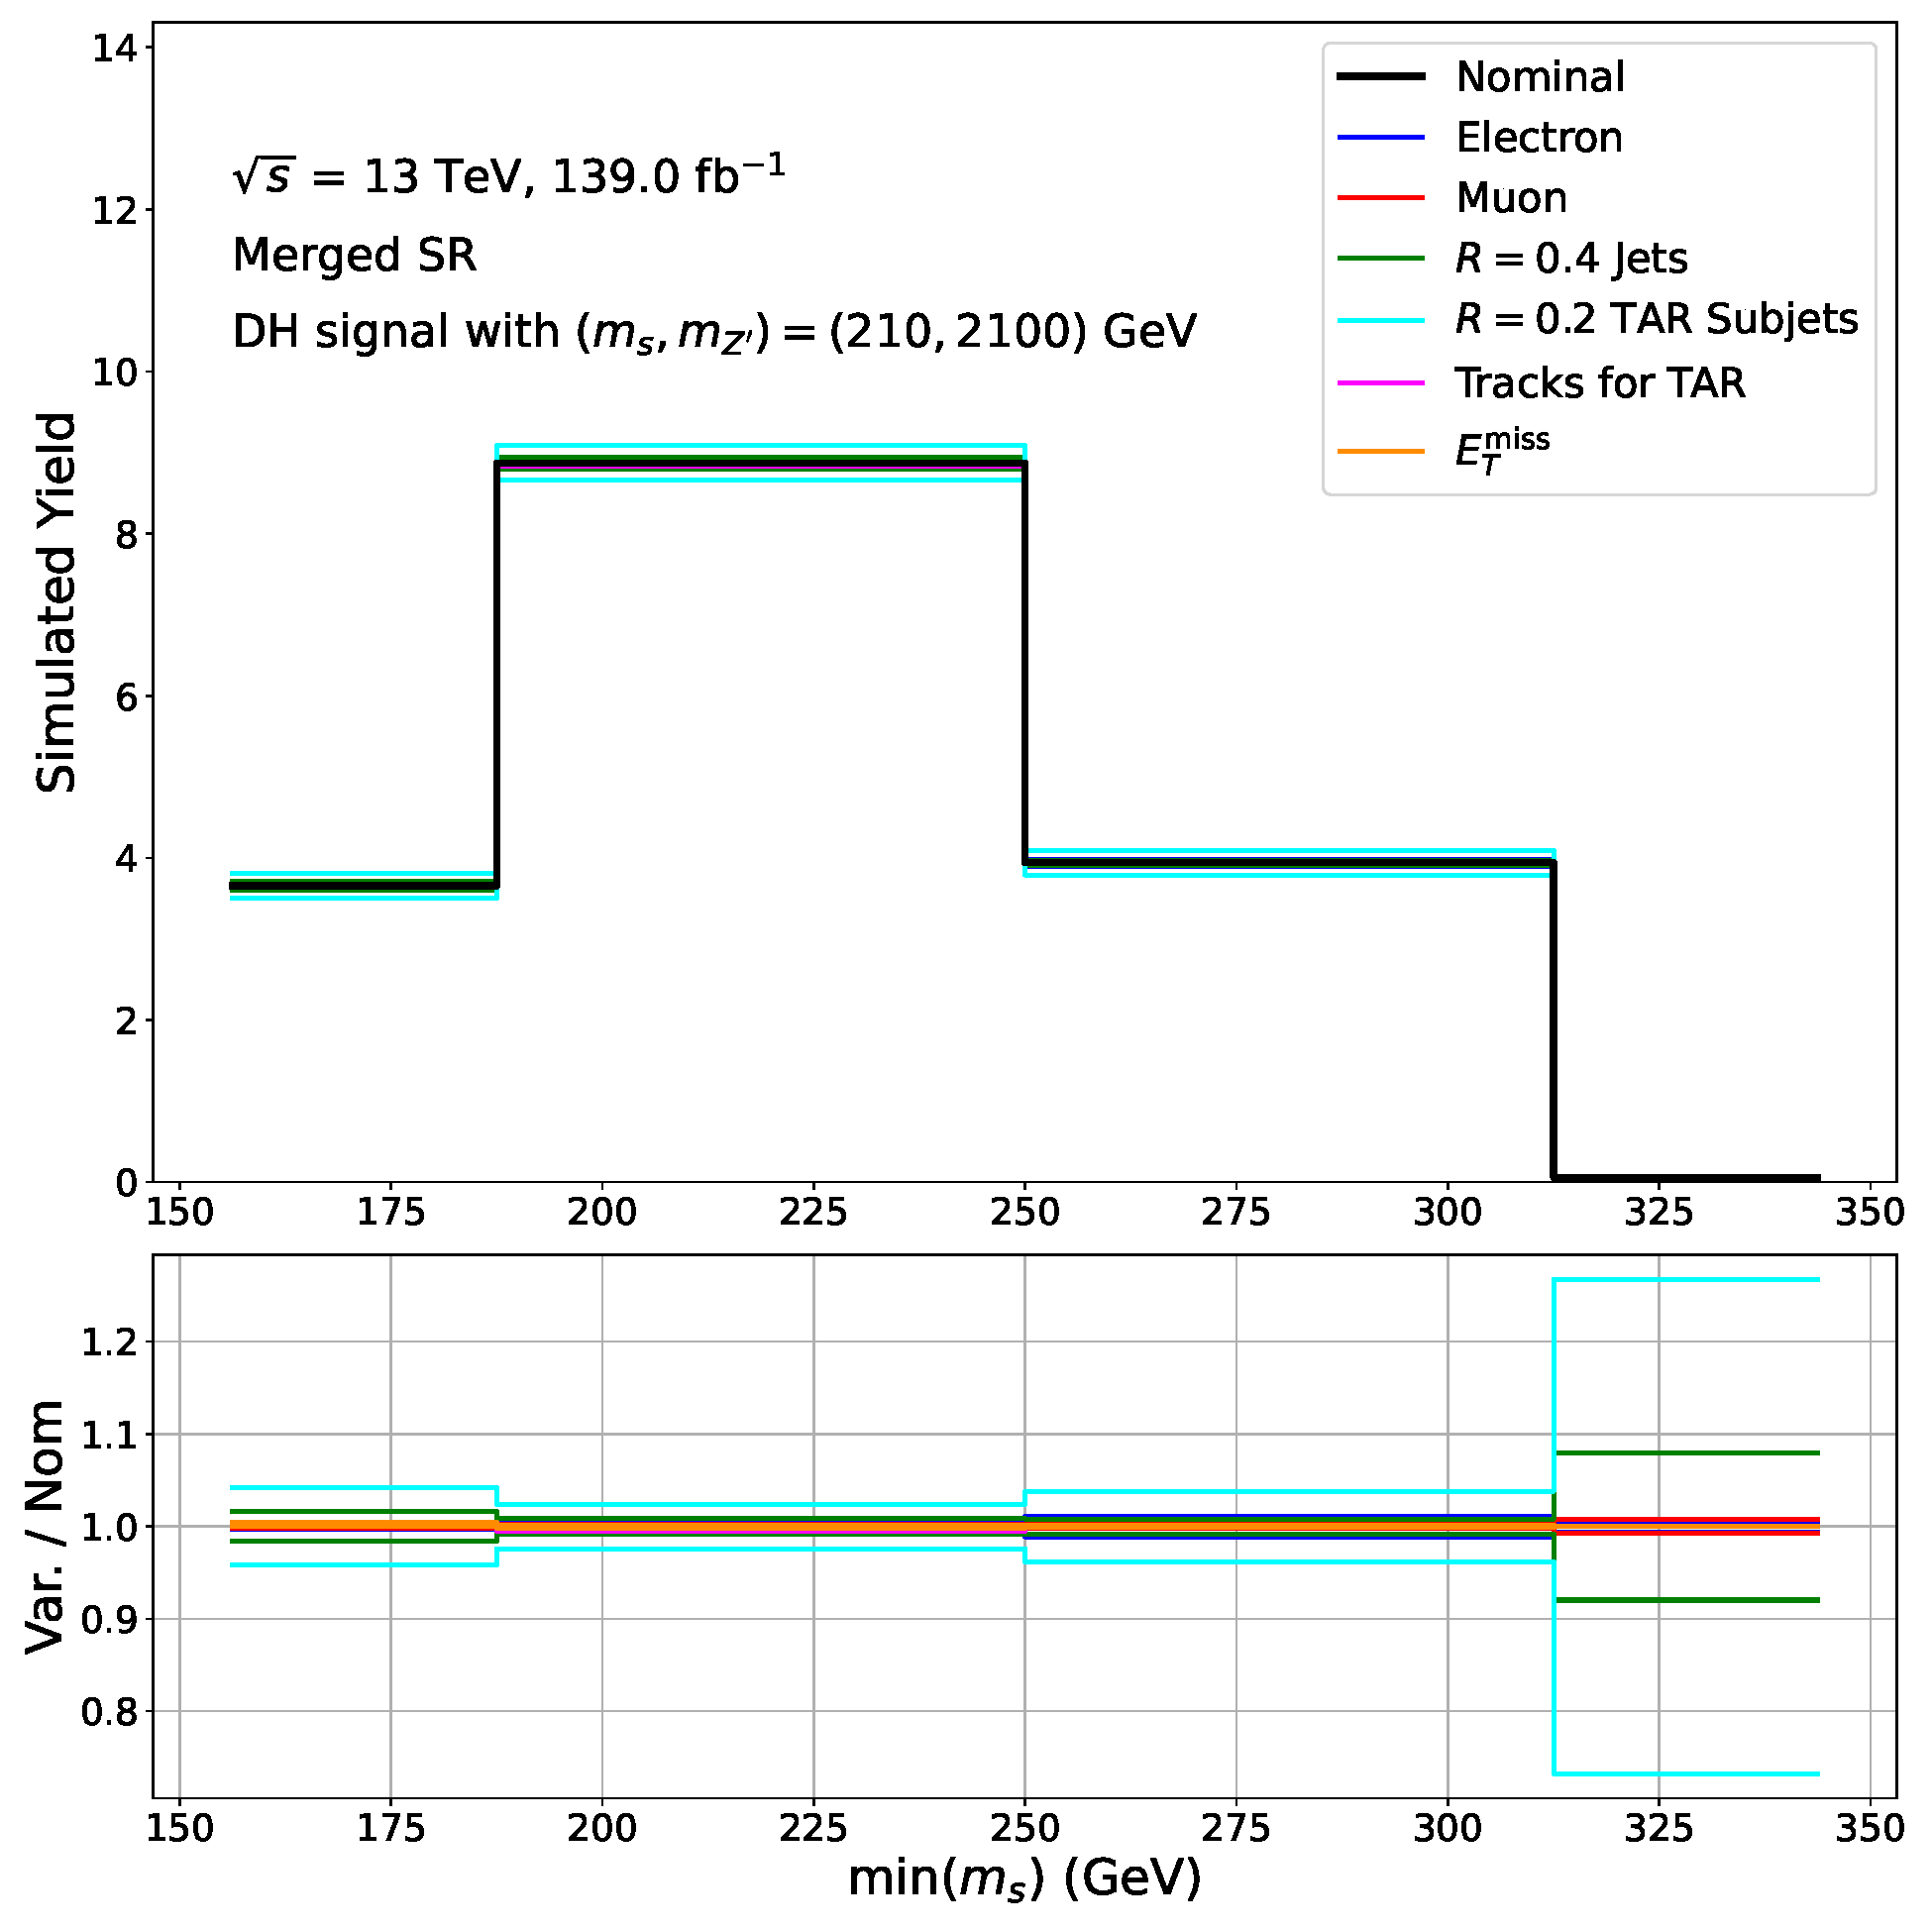
\includegraphics[width = 0.99\textwidth]{Figures/6/exp_systs_monoSWWsemilep_zp2100_dm200_dh210_SR_mgd_TARJets10_minmS_mgd.pdf}
    \caption{Merged SR}
    \end{subfigure}
    \begin{subfigure}[t]{0.48\textwidth}
    \centering
     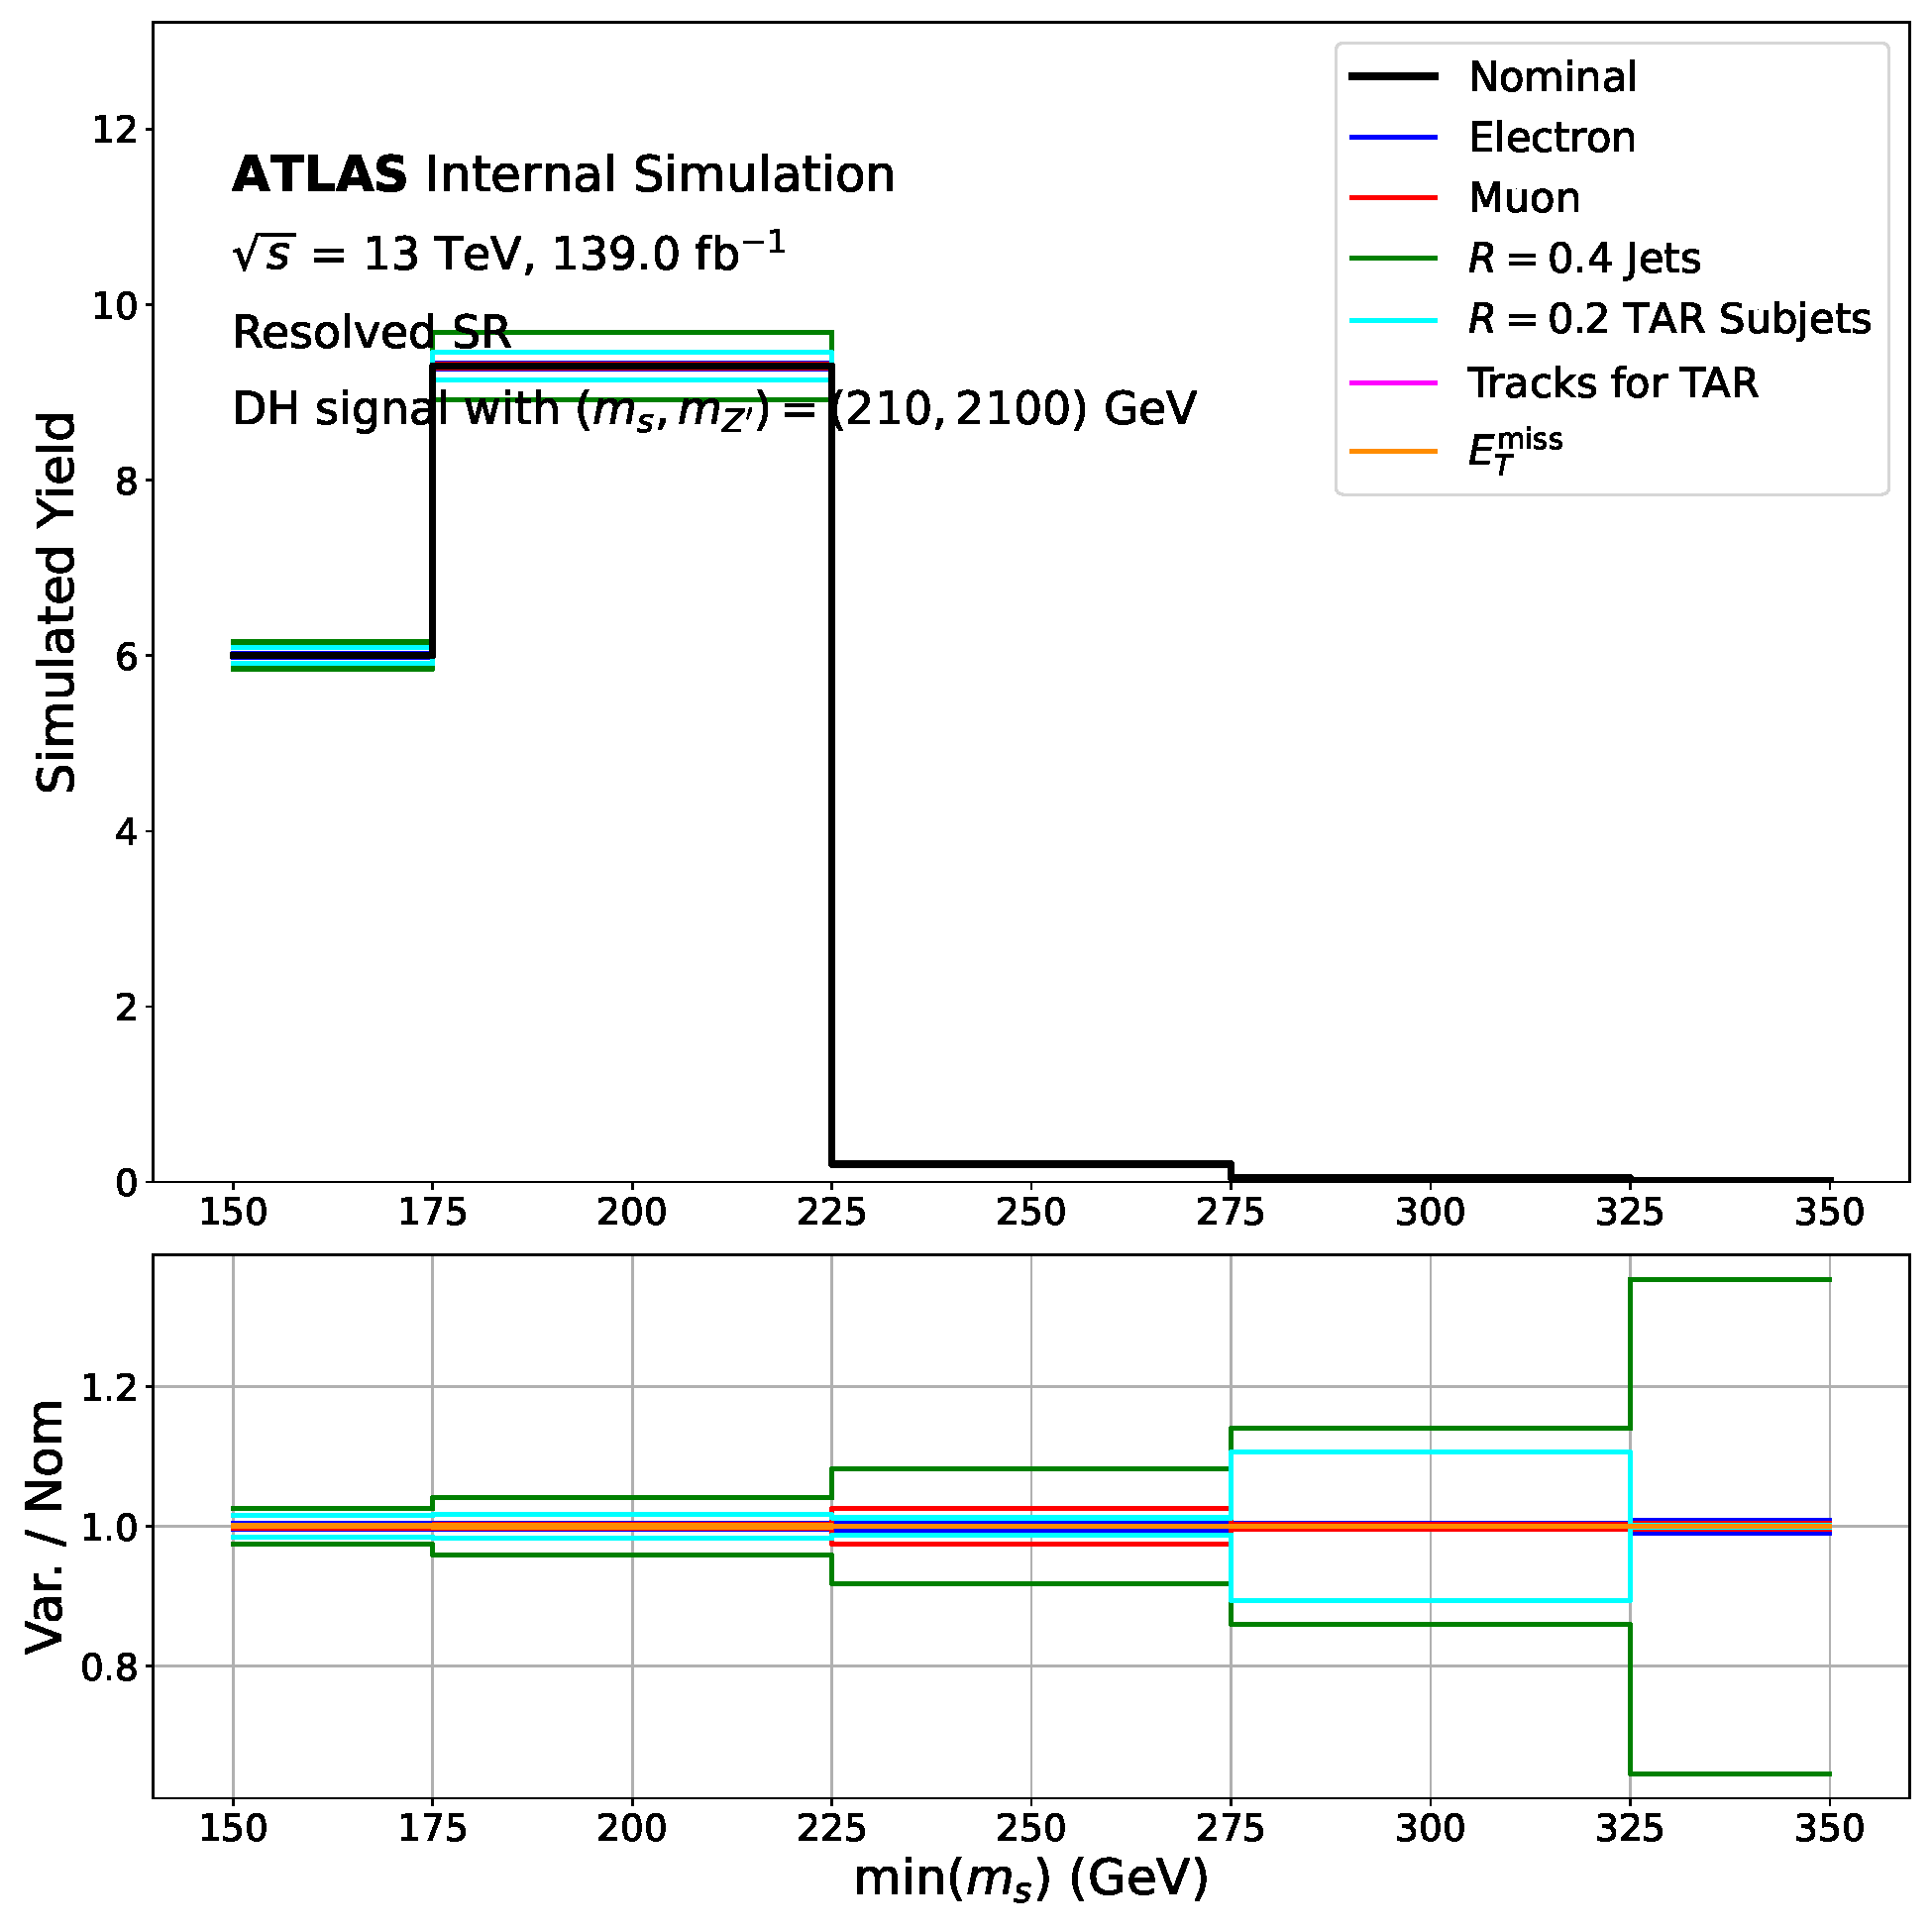
\includegraphics[width = 0.99\textwidth]{Figures/6/exp_systs_monoSWWsemilep_zp2100_dm200_dh210_SR_res_TARJets10_minmS_res.pdf}
     \caption{Resolved SR}
    \end{subfigure}
    \caption{Envelope of shifts in the predicted yield of the DH signal process at \((\ms, \mZp)=(210, 2100)\) in the merged (left) and resolved (right) SRs due to experimental systematics associated with each physics object considered in the search. The predicted yield is binned in \minms using the binning strategy employed in the fit used to search for evidence of the DH signal model in the data (see Chapter \ref{chapter:stat} for details). Bottom panel shows ratio of the shifts relative to the nominal yield. }
   \label{fig:exp_syst_shifts_sig}
\end{figure}

Tables \ref{tab:systs_total_bkg_JET_JER_SR} and \ref{tab:systs_total_bkg_JET_JER_CR} show a sample breakdown of systematic uncertainties associated with the total predicted yield of SM background processes in the SRs and CRs, respectively, which arise from shifting uncertain parameters associated with the reconstructed jet energy resolution (JER) of \(R=0.4\) jets by \(\pm\sigma\). The \(R=0.4\) JER systematics are shown because they produce relatively large shifts in predicted yields compared with other experimental sources.

\begin{table}[ht]
\caption{\label{tab:systs_total_bkg_JET_JER_SR} Symmetrized up and down uncertainties in total predicted yield of all SM background processes in the merged and resolved SRs due to varying parameters associated with jet energy resolution (JER) by \(\pm1\sigma\). Uncertainties are reported as percent shift relative to nominal yield.}
\footnotesize{
\begin{tabular}{l l l l l }
\toprule
\textbf{Name of JER parameter} & \textbf{Mgd SR} & \textbf{Res SR}\tabularnewline
\midrule
\midrule
JET\_JER\_DataVsMC\_MC16 & \(\pm\)6.09\% &\(\pm\)1.17\% \tabularnewline
\midrule
JET\_JER\_EffectiveNP\_1 & \(\pm\)8.74\% &\(\pm\)0.07\% \tabularnewline
\midrule
JET\_JER\_EffectiveNP\_2 & \(\pm\)2.62\% &\(\pm\)2.73\% \tabularnewline
\midrule
JET\_JER\_EffectiveNP\_3 & \(\pm\)0.48\% &\(\pm\)0.87\% \tabularnewline
\midrule
JET\_JER\_EffectiveNP\_4 & \(\pm\)0.83\% &\(\pm\)1.66\% \tabularnewline
\midrule
JET\_JER\_EffectiveNP\_5 & \(\pm\)4.59\% &\(\pm\)3.70\% \tabularnewline
\midrule
JET\_JER\_EffectiveNP\_6 & \(\pm\)7.59\% &\(\pm\)2.44\% \tabularnewline
\midrule
JET\_JER\_EffectiveNP\_7restTerm & \(\pm\)2.96\% &\(\pm\)0.60\% \tabularnewline
\bottomrule
\end{tabular}}
\end{table}

\begin{table}[ht]
\caption{\label{tab:systs_total_bkg_JET_JER_CR} Symmetrized up and down uncertainties in total predicted yield of all SM background processes in the merged and resolved CRs due to varying parameters associated with jet energy resolution (JER) by \(\pm1\sigma\). Uncertainties are reported as percent shift relative to nominal yield.}
\footnotesize{
\begin{tabular}{l l l l l }
\toprule
\textbf{Name of JER parameter} & \textbf{Mgd CRW} & \textbf{Res CRW} & \textbf{Mgd CRTT} & \textbf{Res CRTT}\tabularnewline
\midrule
\midrule
JET\_JER\_DataVsMC\_MC16 & \(\pm\)0.42\% &\(\pm\)0.98\% &\(\pm\)1.25\% &\(\pm\)1.57\% \tabularnewline
\midrule
JET\_JER\_EffectiveNP\_1 & \(\pm\)0.75\% &\(\pm\)0.68\% &\(\pm\)1.07\% &\(\pm\)4.50\% \tabularnewline
\midrule
JET\_JER\_EffectiveNP\_2 & \(\pm\)0.77\% &\(\pm\)0.82\% &\(\pm\)0.73\% &\(\pm\)6.47\% \tabularnewline
\midrule
JET\_JER\_EffectiveNP\_3 & \(\pm\)0.56\% &\(\pm\)1.31\% &\(\pm\)1.05\% &\(\pm\)4.10\% \tabularnewline
\midrule
JET\_JER\_EffectiveNP\_4 & \(\pm\)0.89\% &\(\pm\)2.91\% &\(\pm\)0.13\% &\(\pm\)4.09\% \tabularnewline
\midrule
JET\_JER\_EffectiveNP\_5 & \(\pm\)0.55\% &\(\pm\)0.61\% &\(\pm\)0.24\% &\(\pm\)6.29\% \tabularnewline
\midrule
JET\_JER\_EffectiveNP\_6 & \(\pm\)0.03\% &\(\pm\)1.61\% &\(\pm\)0.32\% &\(\pm\)5.69\% \tabularnewline
\midrule
JET\_JER\_EffectiveNP\_7restTerm & \(\pm\)0.21\% &\(\pm\)1.72\% &\(\pm\)0.03\% &\(\pm\)4.29\% \tabularnewline
\bottomrule
\end{tabular}}
\end{table}

\section{Theoretical Systematics}

The sources of theoretical uncertainty considered in this search, as well as the methods used to evaluate the resulting uncertainties in predicted yields for the various processes relevant to the search, are discussed in the following sections. Some sources are only evaluated for a subset of the processes considered in the search.

Table \ref{tab:theo_sys_summary} summarizes the theoretical uncertainties that are evaluated for each process\footnote{Due the relatively low yield and small number of MC simulated events admitted into the analysis regions for the \zjets process and the similarity in the production mechanisms for the \wjets and \zjets processes, theoretical uncertainties are not explicitly calculated for the \zjets process. Instead, all relative theoretical uncertainties evaluated in each bin \(j\) for the \wjets process \(\text{syst}\text{(theo unc, \wjets, \(j\))} / N_\text{\wjets, nominal, \(j\)}\) are also assigned to the \zjets process.}.

\begin{table}
\centering
\caption{Summary of theoretical uncertainties evaluated for each process considered in the search.}
\label{tab:theo_sys_summary}
%\begin{tabular}{l p{6cm} l l }
\footnotesize{
\begin{tabular}{l l l l l l l l }
\toprule
\textbf{Source} & \textbf{W+jets} & \textbf{Diboson} & \textbf{Triboson} & \textbf{Z+jets} & \(\mathbf{\ttbar}\) & \textbf{Single Top} & \textbf{DH Signal} \\
\midrule
\midrule
PDF & \checkmark & \checkmark & \checkmark & \checkmark & \checkmark & \checkmark & \checkmark \\
\midrule
\(\alpha_s\) (PDF) & \checkmark & \checkmark & \checkmark & \checkmark & \(\times\) & \(\times\) & \(\times\) \\
\midrule
\(\alpha_s\) (ISR) & \(\times\) & \(\times\) & \(\times\) & \(\times\) & \checkmark & \checkmark & \(\times\) \\
\midrule
\(\mu_R\) and \(\mu_F\) & \checkmark & \checkmark & \checkmark & \checkmark & \checkmark & \checkmark & \checkmark \\
\midrule
ME & \(\times\) & \(\times\) & \(\times\) & \(\times\) & \checkmark & \checkmark & \(\times\) \\
\midrule
PS & \checkmark & \checkmark & \checkmark & \checkmark & \checkmark & \checkmark & \checkmark \\
\midrule
\(Wt\)/\ttbar Int. & \(\times\) & \(\times\) & \(\times\) & \(\times\) & \(\times\) &  \checkmark & \(\times\) \\
\bottomrule
\end{tabular}}
\end{table}

\subsection{Use of Acceptance for Evaluating Theoretical Systematics of the DH Signal Model}

For the SM background processes, the systematic uncertainties of predicted yields due to theoretical sources are in general evaluated directly using yield shifts induced by varying the uncertain parameter. Following ATLAS guidelines, theoretical uncertainties associated with the modelling of the DH signal process are instead evaluated in a given bin by calculating the relative shift in the so-called ``acceptance". The acceptance is defined for a given process \(p\) as the ratio of yield in the given bin with all analysis selection applied, relative to the inclusive yield of the process with no selections applied:

\begin{equation}
\label{eq:acceptance}
\text{acc(p, \text{ bin } j)} = \frac{N(p, j)}{N(p, \text{inclusive})}
\end{equation}

The uncertainty in the predicted yield in each bin is then evaluated by multiplying the relative shift in acceptance by the nominal yield in the bin:

\begin{equation}
\label{eq:yield_unc_from_acceptance}
\text{syst\text{(\(p\), up, bin \(j\))}} = N_\text{\(p\), nom, \(j\)} \Bigg(\frac{\text{acc(\(p\), up, \(j\))} - \text{acc(\(p\), nom, \(j\))}}{\text{acc(\(p\), nom, \(j\))}}\Bigg)
\end{equation}

Unless a given uncertainty applies exclusively to the signal model, the methods used to evaluate the uncertainties in the yield associated with each theoretical source are for the sake of brevity presented in their direct application to the yield, as would be used for background processes. In general, the presented methods would be applied rather to the acceptance when considering the DH signal process, and the yield uncertainty would subsequently be derived from the relative acceptance uncertainty using Eq. \ref{eq:yield_unc_from_acceptance}.

\subsection{Modelling the Parton Distribution Function}
\label{sec:pdf_unc}

Uncertainties associated with the parton distribution function\footnote{See Section \ref{sec:parton_model} for an introduction to the parton model and parton distribution functions.} (PDF) used to model the substructure of protons involved in LHC collisions can affect the predicted cross sections of production and decay processes at the LHC. Following ATLAS guidelines and recommendations from the \textit{PDF4LHC} \cite{PDF4LHC_recos_2016} working group, generator weights\footnote{See discussion of generator weights in Section \ref{sec:evt_wts}} of events simulated for all processes are re-evaluated for 100 replicas of the nominal PDF. Each replica is obtained by randomly re-sampling all uncertain inputs to the PDF model and re-evaluating the PDF with the new inputs \cite{BALL20091}. The yield in each region and bin is re-evaluated with each set of generator weights, and the uncertainty of the yield in each bin for a given process is estimated as the standard deviation over all yield variations \cite{PDF4LHC_recos_2016}.

\subsection{Strong Coupling Constant \(\alpha_s\)}

The nominal PDF is produced with the strong coupling constant \(\alpha_s\) set to its currently accepted value of \(\alpha_s(m_Z^2)=0.1180\pm0.0015\) \cite{PDF4LHC_recos_2016} at a momentum scale \(m_Z\). 

\subsubsection{\(\alpha_s\) in PDF Modelling}

For the \wjets, diboson and triboson processes generated using \SHERPA2.2, alternative generator weights are produced using PDFs re-evaluated with \(\alpha_s\) varied up or down by its \(\pm0.0015\) uncertainty. Following the \textit{PDF4LHC} prescription, the yield \(N_p\) for a given process \(p\) is re-evaluated in each bin \(j\) with the alternative generator weights, and the uncertainty is evaluated as:

\begin{equation}
\label{eq:alphas_syst}
\text{syst}\text{(\(\alpha_s\), \(p\), bin \(j\))}= \pm\Bigg(\frac{N_\text{\(p\), \(\alpha_s\)+1\(\sigma\), \(j\)} - N_\text{\(p\), \(\alpha_s\)-1\(\sigma\), \(j\)} }{2}\Bigg)
\end{equation}

\noindent and added in quadrature with the PDF uncertainties discussed in Section \ref{sec:pdf_unc}.

\subsubsection{Strong Coupling Constant in the Modelling of Initial State Radiation (ISR)}

For the single-top and \ttbar processes generated using the \POWHEGBOX matrix element generator interfaced with the \PYTHIA8 parton shower generator, the effect of varying the strong \(\alpha_s\) used to model initial state radiation (ISR) from \(\alpha_{s,\text{ ISR}}=0.1\) to \(\alpha_{s, \text{ ISR}}=0.15\) is evaluated using the up and down Var3c A14 tune variation \cite{ATL-PHYS-PUB-2014-021}, and the associated yield uncertainty in each bin is evaluated as half the resulting difference of yields, as in Eq. \ref{eq:alphas_syst}. 

\subsection{Renormalization and Factorization Scales (\(\mu_R\) and \(\mu_F\)) in QCD}

In the framework of perturbative QCD, the strong coupling constant is expressed as a function of the ``renormalization scale" \(\mu_R\) \cite{PDG_2018}, which is unphysical in the sense that the values of physical observables should be independent of \(\mu_R\). However, the choice of \(\mu_R\) can impact the calculated values of observables in perturbative QCD calculations due to missing higher-order terms in truncated expansions. A similar effect is seen with the ``factorization scale" \(\mu_F\) used in calculations of the proton PDF \cite{maltoni2007choosing}, which effectively quantifies the resolution with which the proton is probed in a collision. As with \(\mu_R\), the choice of \(\mu_F\) has no physical meaning, but affects the calculated values of observables due to missing higher-order terms in truncated QCD expansions.

To account for the unphysical impact of the choice of \(\mu_R\) and \(\mu_F\) on simulated observables, generator weights are re-evaluated for each process with \(\mu_R\) and \(\mu_F\) varied by factors of either \(\frac{1}{2}\) or 2 in pairwise combinations (i.e. \((\mu_R, \mu_F)\rightarrow \{(\frac{1}{2}\mu_R, \mu_F), (\mu_R, 2\mu_F)\}\), etc.) from their values used for the nominal event generation. Following ATLAS guidelines, the systematic uncertainty in the yield in each bin is evaluated as the envelope of yield variations over all pairwise combinations of \(\mu_R\) and \(\mu_F\) variations, excluding the extreme off-diagonals \(\{(\frac{1}{2}\mu_R, 2\mu_F), (2\mu_R, \frac{1}{2}\mu_F)\}\): 
%For a given process \(p\), the upward systematic uncertainty of the predicted yield \(N_p\) for process \(p\) in bin \(j\) is evaluated as:

\begin{equation}
\label{eq:scale_systs}
\text{syst}\text{(scale, up, \(p\), bin \(j\))} = \max\bigg[0, \max\limits_{k\in\{\mu_R, \mu_F \text{ var'ns}\}} \big\{N_\text{\(p\), \(k\), \(j\)} - N_\text{\(p\), nom, \(j\)}\big\} \bigg]
\end{equation}

\noindent where ``max"\(\rightarrow\)``min" for the ``down" variation.

\subsection{Matrix Element (ME) Generator Comparison}
\label{sec:ME_syst}

For the \ttbar and single-top processes, for which separate generators are used to calculate the ME (\POWHEGBOX) for the hard scatter process and model the subsequent parton shower (\PYTHIA8), an uncertainty associated with the choice of \POWHEGBOX used to calculate the ME is obtained by comparing the nominal yield predictions with those obtained using an alternate MadGraph5\_aMC\@NLO \cite{Alwall:2014hca} generator. The associated uncertainty in the predicted yield for a given process \(p\) (\ttbar or single-top) in bin \(j\) is evaluated using the difference in yield obtained with the alternate ME calculator:

\begin{equation}
\label{eq:ME_syst}
\text{syst}\text{(ME, \(p\), bin \(j\))}= \pm \Big(N_\text{\(p\), ME=MadGraph5\_aMC\@NLO, \(j\)} - N_\text{\(p\), nom, \(j\)}\Big)
\end{equation}

\subsection{Parton Showering (PS)}

Uncertainties associated with the modelling of the PS are evaluated for all processes. The approach used to evaluate these uncertainties for a given process differs depending on which package, or set of packages, was used to generate the nominal set of MC simulated events for the process.

\subsubsection{Alternate PS Generator}

For the \ttbar, single-top and DH signal processes for which separate packages are used to calculate the ME and to model the subsequent PS, an uncertainty associated with the choice of PS generator is evaluated by comparing the predicted yields obtained with the nominal \PYTHIA8 PS generator with an alternate \HERWIG[7] \cite{Bahr:2008pv,Bellm:2015jjp} generator. In analogy with the evaluation of ME uncertainty described in Section \ref{sec:ME_syst} above, the associated uncertainty in yield is evaluated for the \ttbar and single-top processes as:

\begin{equation}
\label{eq:ME_syst}
\text{syst}\text{(PS, \(p\), bin \(j\))}= \pm \Big(N_\text{\(p\), PS=\HERWIG[7], \(j\)} - N_\text{\(p\), nom, \(j\)}\Big)
\end{equation}

For the DH signal model, MC simulated samples are generated with the alternate \HERWIG[7] PS generator at three sample points in \ms and \mZp:

\begin{itemize}
\item \((\ms, m_{Z'}) = (160, 1000)~\GeV\)
\item \((\ms, m_{Z'}) = (160, 2100)~\GeV\)
\item \((\ms, m_{Z'}) = (310, 1000)~\GeV\)
\end{itemize}

For each choice of PS generator - nominal or alternate - all three sets of samples generated at the mass points listed above are statistically combined, with the cross section excluded from the event weights\footnote{see Section \ref{sec:evt_wts} for a detailed discussion of event weights}. The cross section is excluded when combining the samples to prevent the signal points at \(\ms=160~\GeV\) with larger cross sections from dominating the shape of the combined sample. Using the combined DH sample, the relative uncertainty in the predicted acceptance associated with the alternate PS generator is evaluated as:

\begin{small}
\begin{equation}
\label{eq:ME_syst}
\text{(rel. syst)}\text{(PS, comb. DH, bin \(j\))}= \pm \Bigg( \frac{\text{acc}_\text{comb. DH, PS=\HERWIG[7], \(j\)} - \text{acc}_\text{comb. DH, nom, \(j\)}}{\text{acc}_\text{comb. DH, nom, \(j\)}} \Bigg)
\end{equation}
\end{small}

\noindent This relative uncertainty is then applied to the DH signal yields at all \ms and \mZp:

\begin{small}
\begin{equation}
\label{eq:ckkw_wjets}
\text{syst}_\text{(PS, (\ms, \mZp), bin \(j\))} = \pm \bigg[\text{(rel. syst)}\text{(PS, combined DH, \(j\))}\bigg] \times \bigg[N_\text{(\ms, \mZp), nom, \(j\)}\bigg]
\end{equation}
\end{small}

\subsubsection{CKKW and QSF PS Systematics}

For the \wjets, diboson and triboson processes, the \SHERPA2.2 generator is used to model both the ME calculation and the PS. Since it is not in general possible to disentangle the ME and PS components of the \SHERPA2.2 event simulation, the uncertainty associated with the PS shower generation is instead evaluated by varying the following theoretical parameters in the parton showering model implemented in \SHERPA2.2:

\begin{itemize}
\item The ``merging scale" \(Q_\text{cut}\) is used to merge the matrix element associated with partonic emissions with the ensuing parton shower evolution in the CKKW scheme \cite{CKKW_2009,Sherpa1.1_2009}. This merging scale is set to 20 GeV for the nominal event generation. Following ATLAS guidelines, the uncertainty associated with the choice of \(Q_\text{cut}\) is evaluated by producing alternate MC simulated samples with \(Q_\text{cut}\) varied to either \(Q_\text{cut, down}=15~\GeV\) or \(Q_\text{cut, up}=30~\GeV\). 
\item The ``resummation scale" \(\mu_\text{QSF}\) \cite{PDG_2018} is used in modelling parton shower evolution. Following ATLAS guidelines, the uncertainty associated with the choice of \(\mu_\text{QSF}\) is evaluated producing alternate samples with \(\mu_\text{QSF}\) varied by factors of either \(\frac{1}{2}\) or 2.
\end{itemize}

\vspace{1em}
\noindent\textit{Evaluation Strategy for the W+jets Process}
\vspace{1em}

For the \wjets process, event weights associated with up and down variations of the \(Q_\text{cut}\) and \(\mu_\text{QSF}\) scales are evaluated by the method described in Ref. \cite{Vjets_ckkw_qsf} using truth-level\footnote{See Section \ref{sec:MC_ATLAS} for information on the distinction between truth-level and reconstruction-level simulation} MC simulated samples that were generated with each scale variation. These event weights are used to re-evaluate the predicted yield of \wjets events in all regions and bins for each scale variation, and the associated uncertainty is calculated as half the difference in yields between up and down variations:

\begin{equation}
\label{eq:ckkw_wjets}
\text{syst}_\text{(CKKW (QSF), \wjets, bin \(j\))} = \pm\Bigg(\frac{N_\text{\wjets, \(Q_\text{cut}\) up (\(\mu_\text{QSF, up}\)), \(j\)} - N_\text{\wjets, \(Q_\text{cut}\) down (\(\mu_\text{QSF, down}\)), \(j\)} }{2}\Bigg)
\end{equation}

\vspace{1em}
\noindent\textit{Evaluation Strategy for Diboson and Triboson Processes}
\vspace{1em}

For the diboson and triboson processes, predicted yields are evaluated for each truth-level sample of MC simulated diboson events generated with variations of the \(Q_\text{cut}\) and \(\mu_\text{QSF}\) scales, and for the nominal truth-level sample, in a single ``inclusive" region defined by the following selection on truth-level observables:

\begin{itemize}
\item (1 signal muon) or (1 signal electron)
\item (1 or more \(R=1.0\) \largeR jet\footnote{The TAR jets used in the search are by default built at reconstruction level. At truth level, the TAR jets are approximated by \(R=1.0\) jets constructed using the \akt algorithm \cite{akt_algo}.}) or (2 or more \(R=0.4\) jets)
\item \(\met > 150~\GeV\)
\item \(\mtlepmet > 150~\GeV\)
\end{itemize}

The inclusive region is designed to contain all of the analysis regions used in the search, with the lower bounds on \met and \mtlepmet placed as high as possible in order to reflect the kinematics of events in the analysis regions, while still admitting enough simulated events to ensure that statistical yield fluctuations are sub-dominant in comparison to the yield shifts resulting from varying \(Q_\text{cut}\) and \(\mu_\text{QSF}\). Within this inclusive region, the relative uncertainty in yield is evaluated for each set of scale variations as:

\begin{footnotesize}
\begin{equation}
\label{eq:ckkw_wjets}
\text{(rel. syst)}_\text{(CKKW (QSF), diboson)} = \pm\Bigg(\frac{N_\text{diboson (tr.), \(Q_\text{cut}\) up (\(\mu_\text{QSF, up}\)), incl.} - N_\text{diboson (tr.), \(Q_\text{cut}\) down (\(\mu_\text{QSF, down}\)), incl.} }{2\times N_\text{diboson (tr.), nom, incl.}}\Bigg)
\end{equation}
\end{footnotesize}

\noindent The relative uncertainty \(\text{(rel. syst)}_\text{(CKKW (QSF), diboson)}\) is applied to the yield in each analysis region and bin in the reconstruction level diboson and triboson\footnote{The relative CKKW and QSF uncertainty evaluated for the diboson process is also applied to the triboson process because there are currently no MC simulated samples available for the triboson process with \(Q_\text{cut}\) and \(\mu_\text{QSF}\) varied.} samples:

\begin{footnotesize}
\begin{equation}
\label{eq:ckkw_wjets}
\text{syst}_\text{(CKKW (QSF), diboson (triboson), bin \(j\))} = \pm \bigg[\text{(rel. syst)}_\text{(CKKW (QSF), diboson)}\bigg] \times \bigg[N_\text{diboson (triboson), nom, \(j\)}\bigg]
\end{equation}
\end{footnotesize}

\vspace{1em}
\noindent\textit{Combination of CKKW and QSF Systematics}
\vspace{1em}

For each process, the CKKW and QSF systematic uncertainties are combined in quadrature to obtain an overall estimate of the total uncertainty associated with the parton shower modelling.

\subsection{Interference Between single-top \(Wt\) and \ttbar Processes at NLO}

Interference between the mechanisms for single-top (\(Wt\)) and \ttbar production \cite{Wt_interference} is accounted for when simulating the single-top process to obtain an accurate prediction of the combined production rate for the two processes. Two theoretical schemes, diagram removal (DR) and diagram subtraction (DS) have been developed to handle this interference. The DR scheme is used to generate the nominal MC simulated samples for the single-top process, and an uncertainty associated with the choice of interference handling scheme is evaluated by generating alternate samples for the single-top process using the DS scheme. The associated uncertainty in the predicted yield of the single-top process is evaluated in each bin \(j\) as:

\begin{equation}
\label{eq:ME_syst}
\text{syst}\text{(\(Wt\)/\ttbar, single-top, bin \(j\))}= \pm \Big(N_\text{single-top, DS, \(j\)} - N_\text{single-top, nom, \(j\)}\Big)
\end{equation}

\subsection{Shifts in Predicted Yields due to Theoretical Systematic Uncertainties}

Figure \ref{fig:theory_systs} shows yield variations associated with all sources of theoretical uncertainty presented in this section in the merged SR for sample processes. 

\begin{figure}[!tb]
  \centering
    \begin{subfigure}{0.45\textwidth}
    \centering
    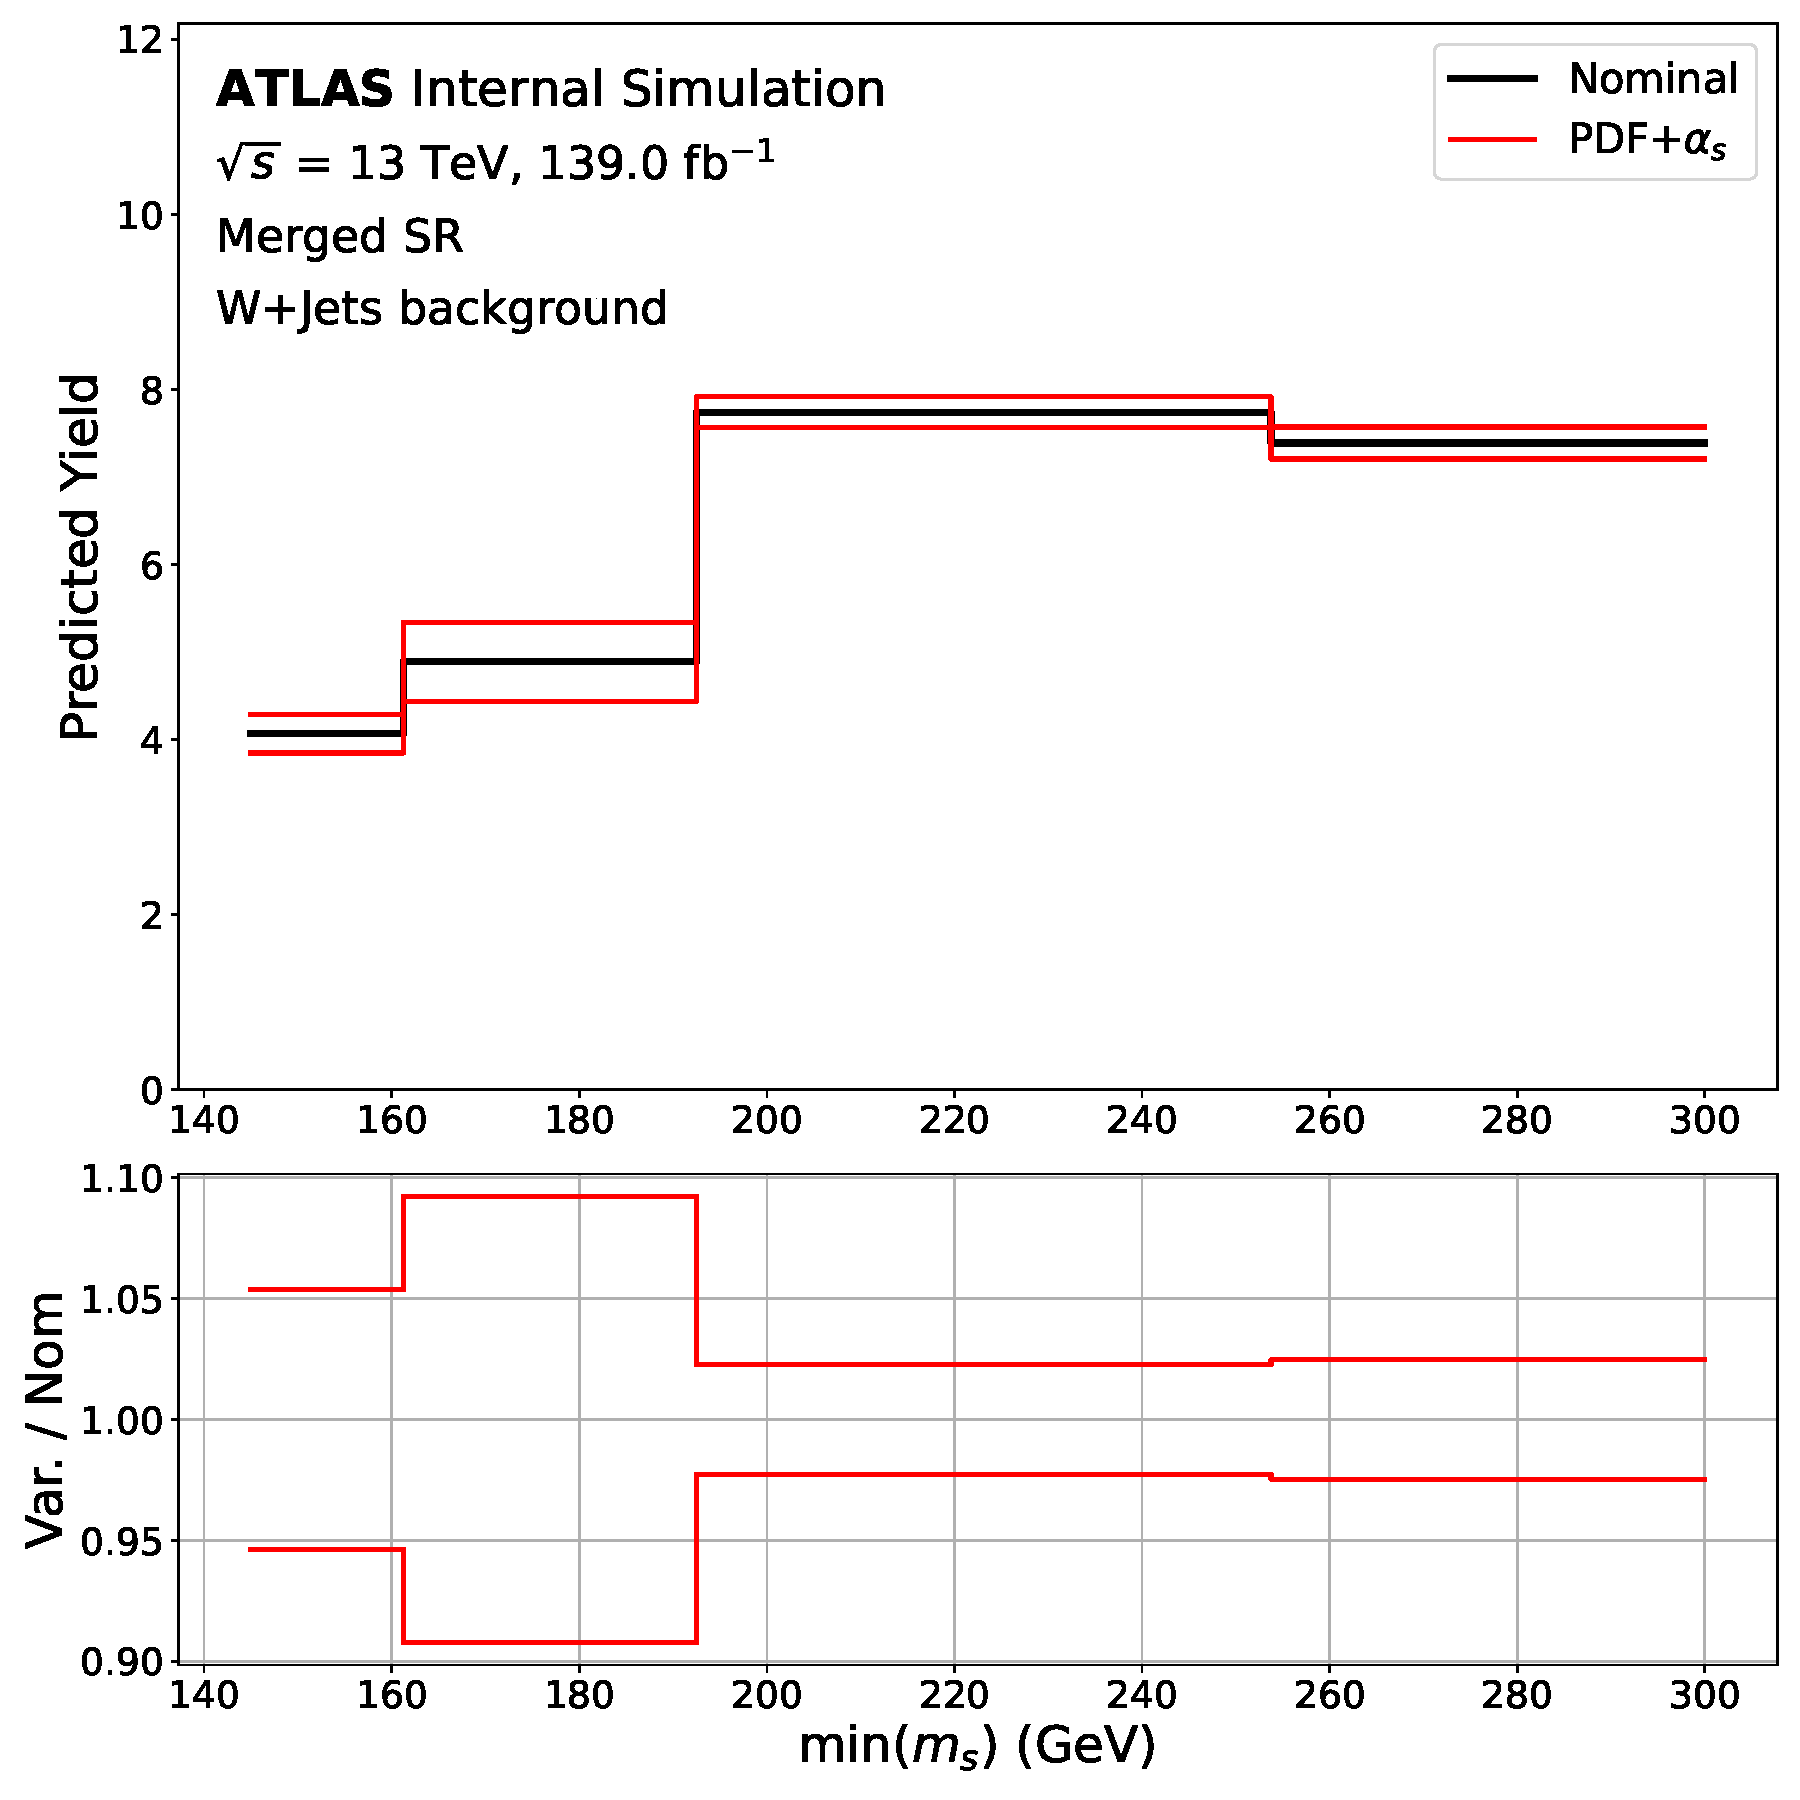
\includegraphics[width=0.9\textwidth]{Figures/6/pdf_plus_alphas_syst_W+Jets_SR_mgd_TARJets10_minmS_mgd_yield.pdf}
    \caption{PDF+\(\alpha_s\) for \wjets background}
    \label{fig:wjets_pdf}
  \end{subfigure} \hspace{1em}
  \begin{subfigure}{0.45\textwidth}
  \centering
    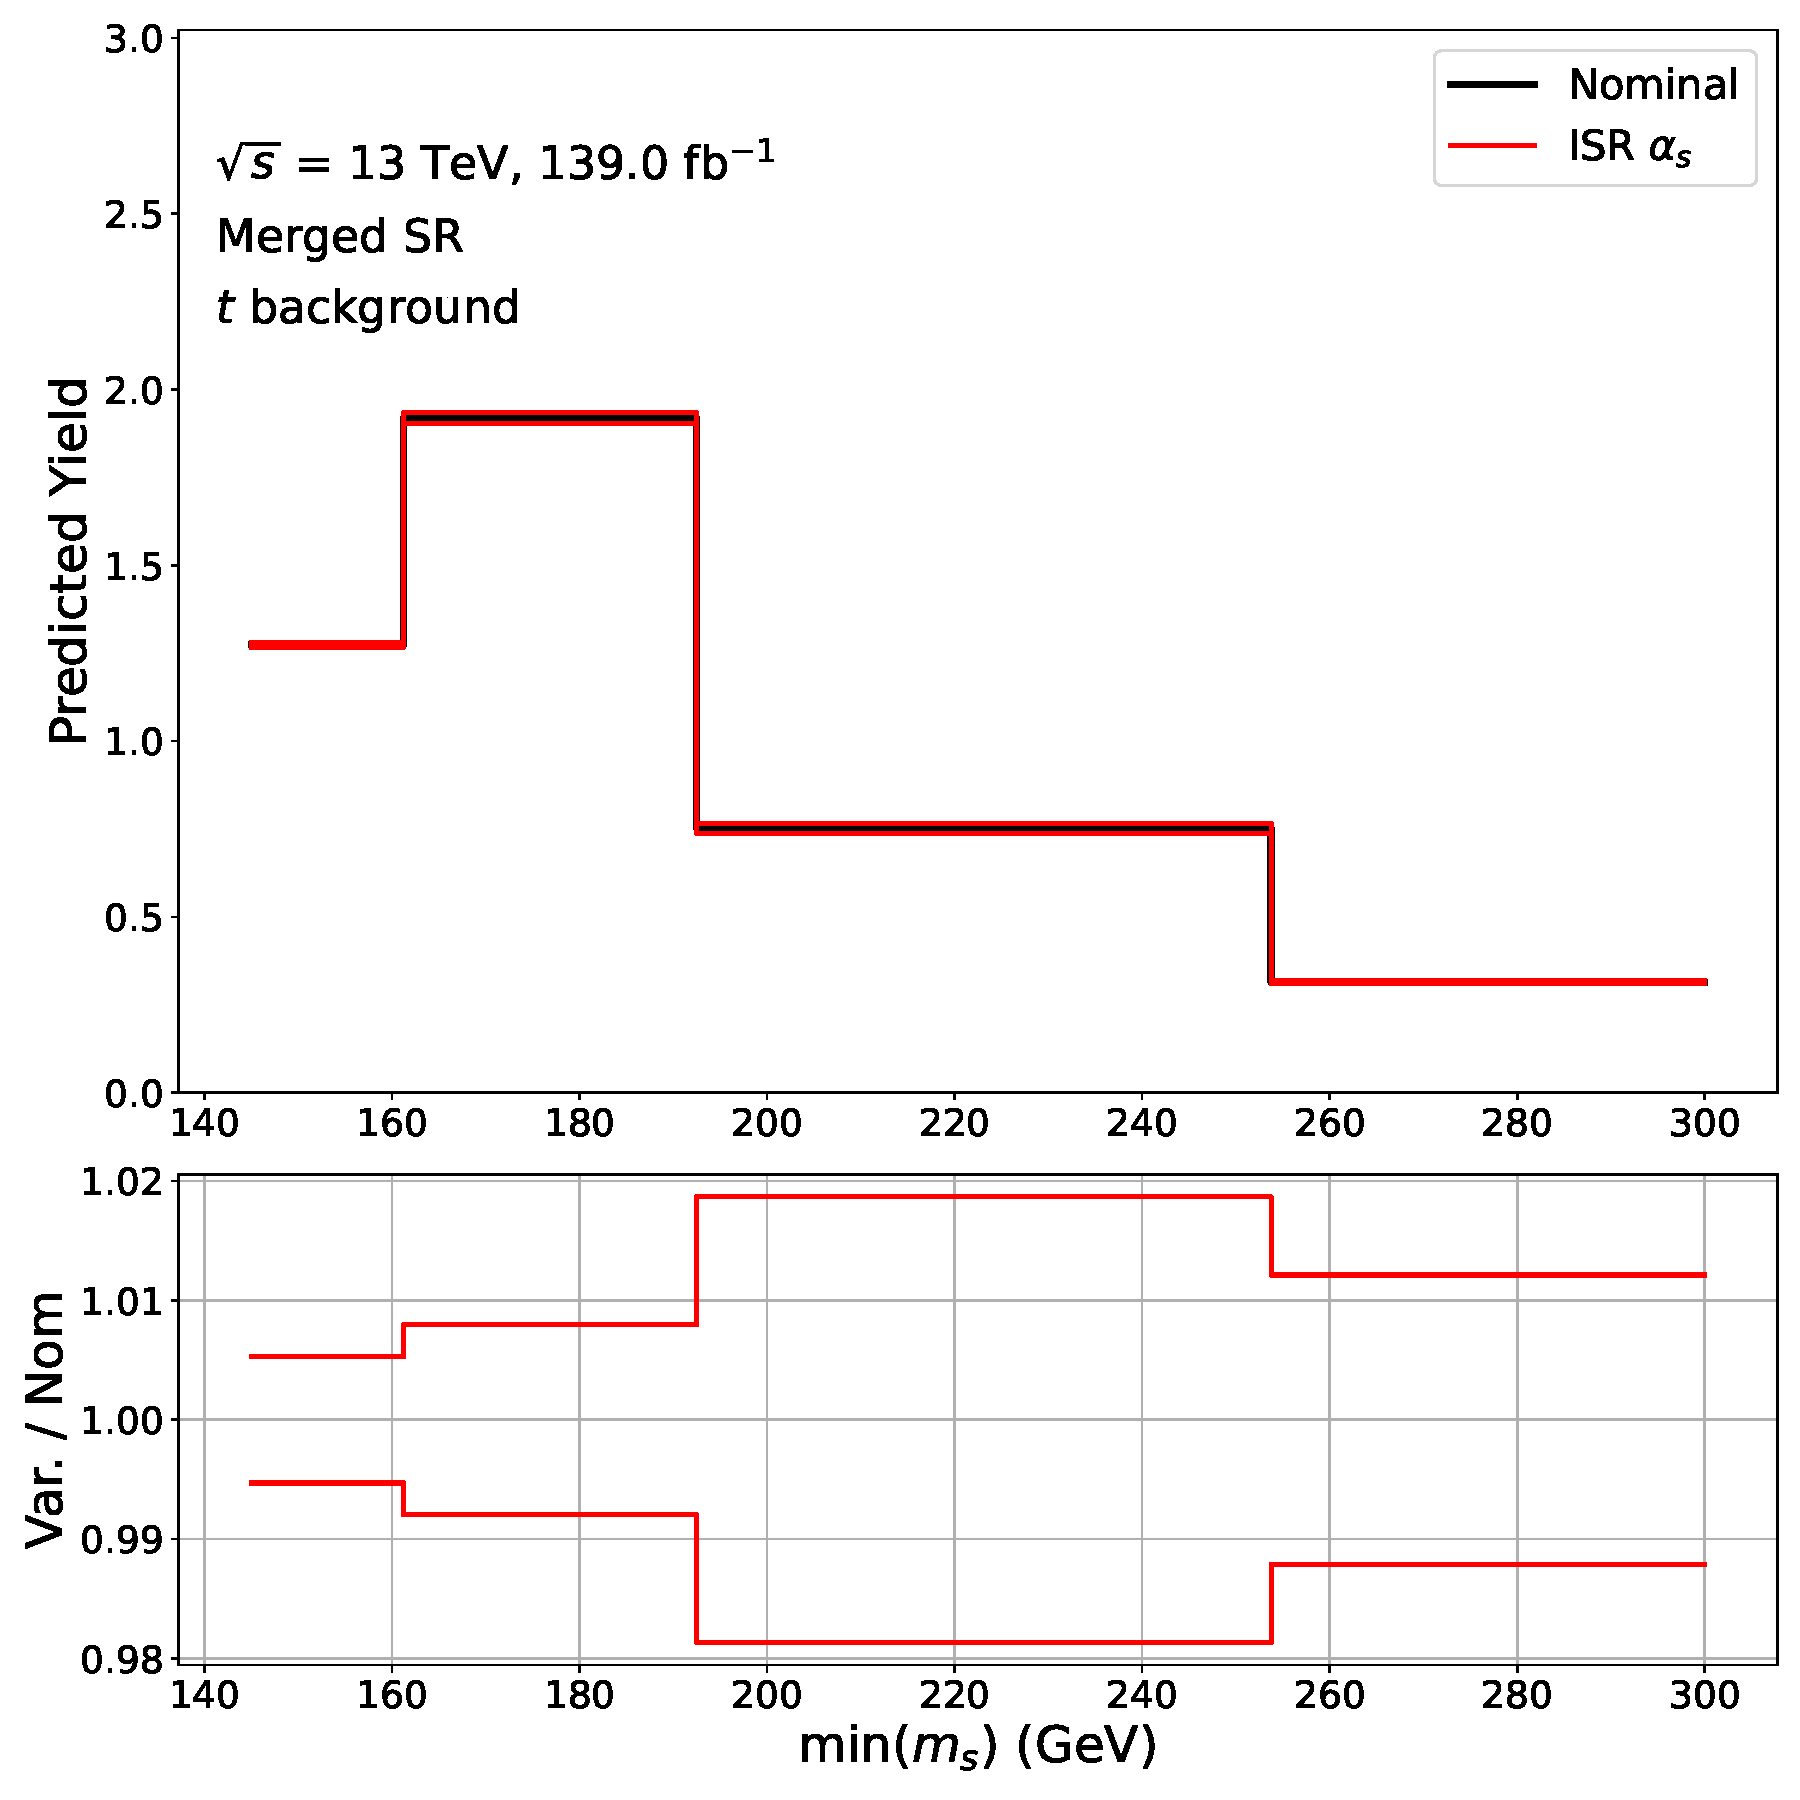
\includegraphics[width=0.9\textwidth]{Figures/6/ISR_alphas_syst_ttbar_SR_mgd_TARJets10_minmS_mgd_yield.pdf}
    \caption{ISR \(\alpha_s\) for \ttbar background}
    \label{fig:ttbar_ISR_alphas}
    \end{subfigure} \\ \vspace{1em}
    
  \begin{subfigure}{0.45\textwidth}
      \centering
    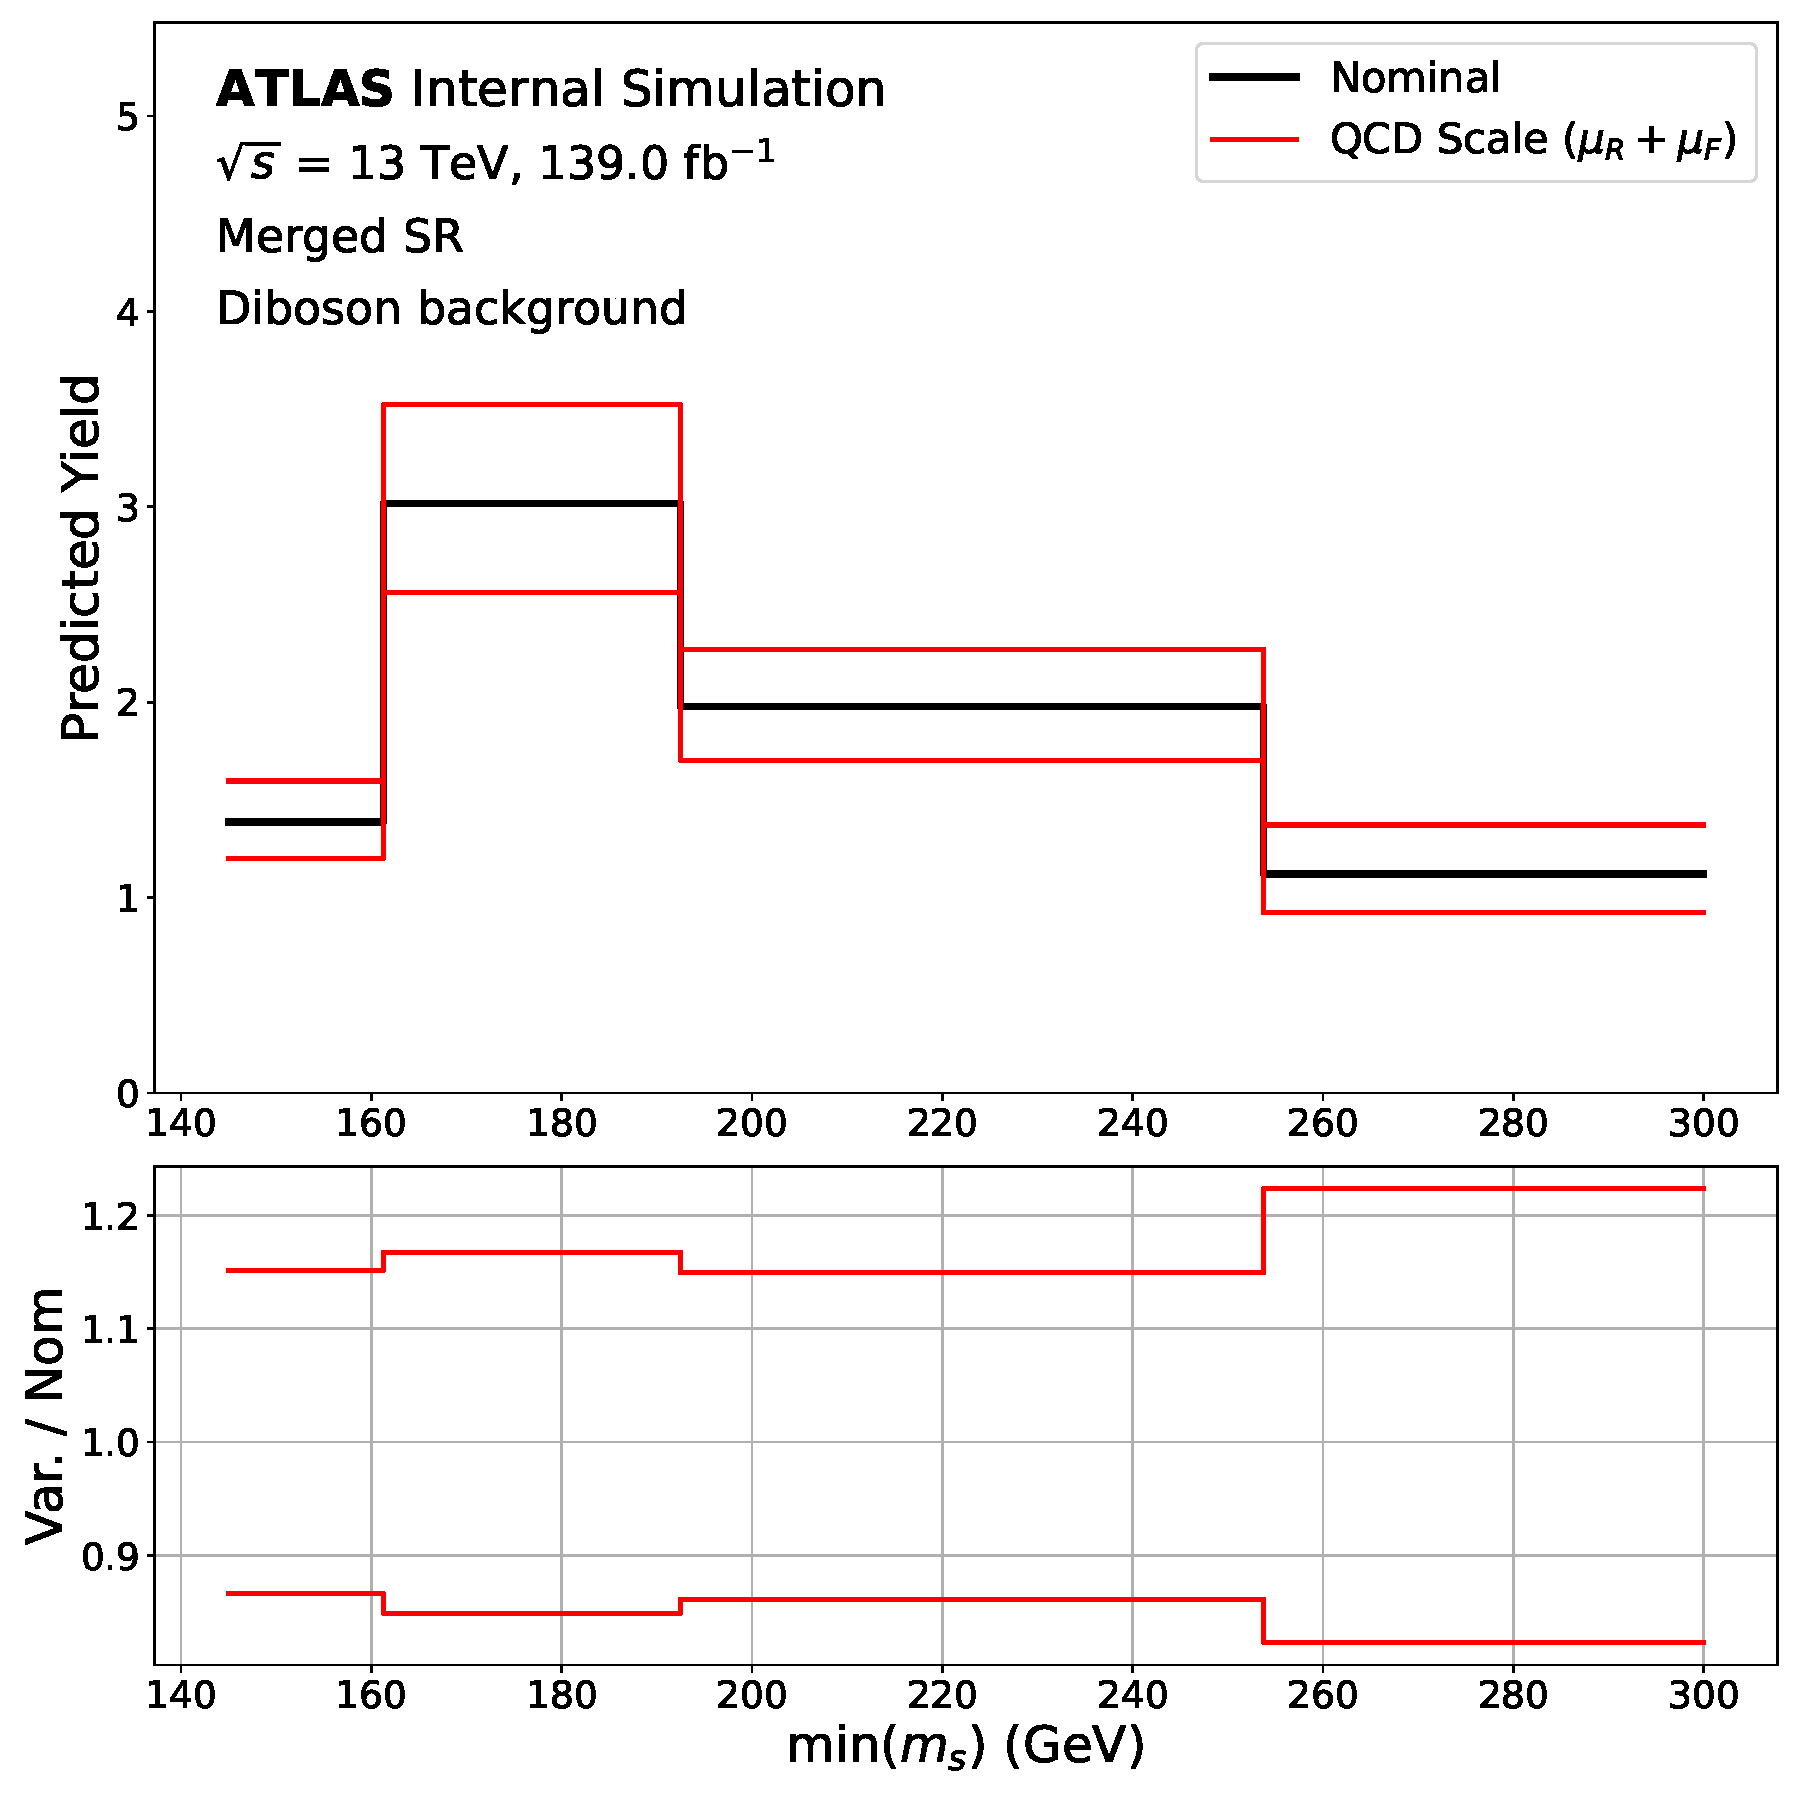
\includegraphics[width=0.9\textwidth]{Figures/6/scale_syst_Diboson_SR_mgd_TARJets10_minmS_mgd_symm_scale_yield.pdf}
    \caption{\(\mu_R+\mu_F\) for diboson background}
    \label{fig:diboson_scale}
  \end{subfigure} \hspace{1em}
      \centering
    \begin{subfigure}{0.45\textwidth}
    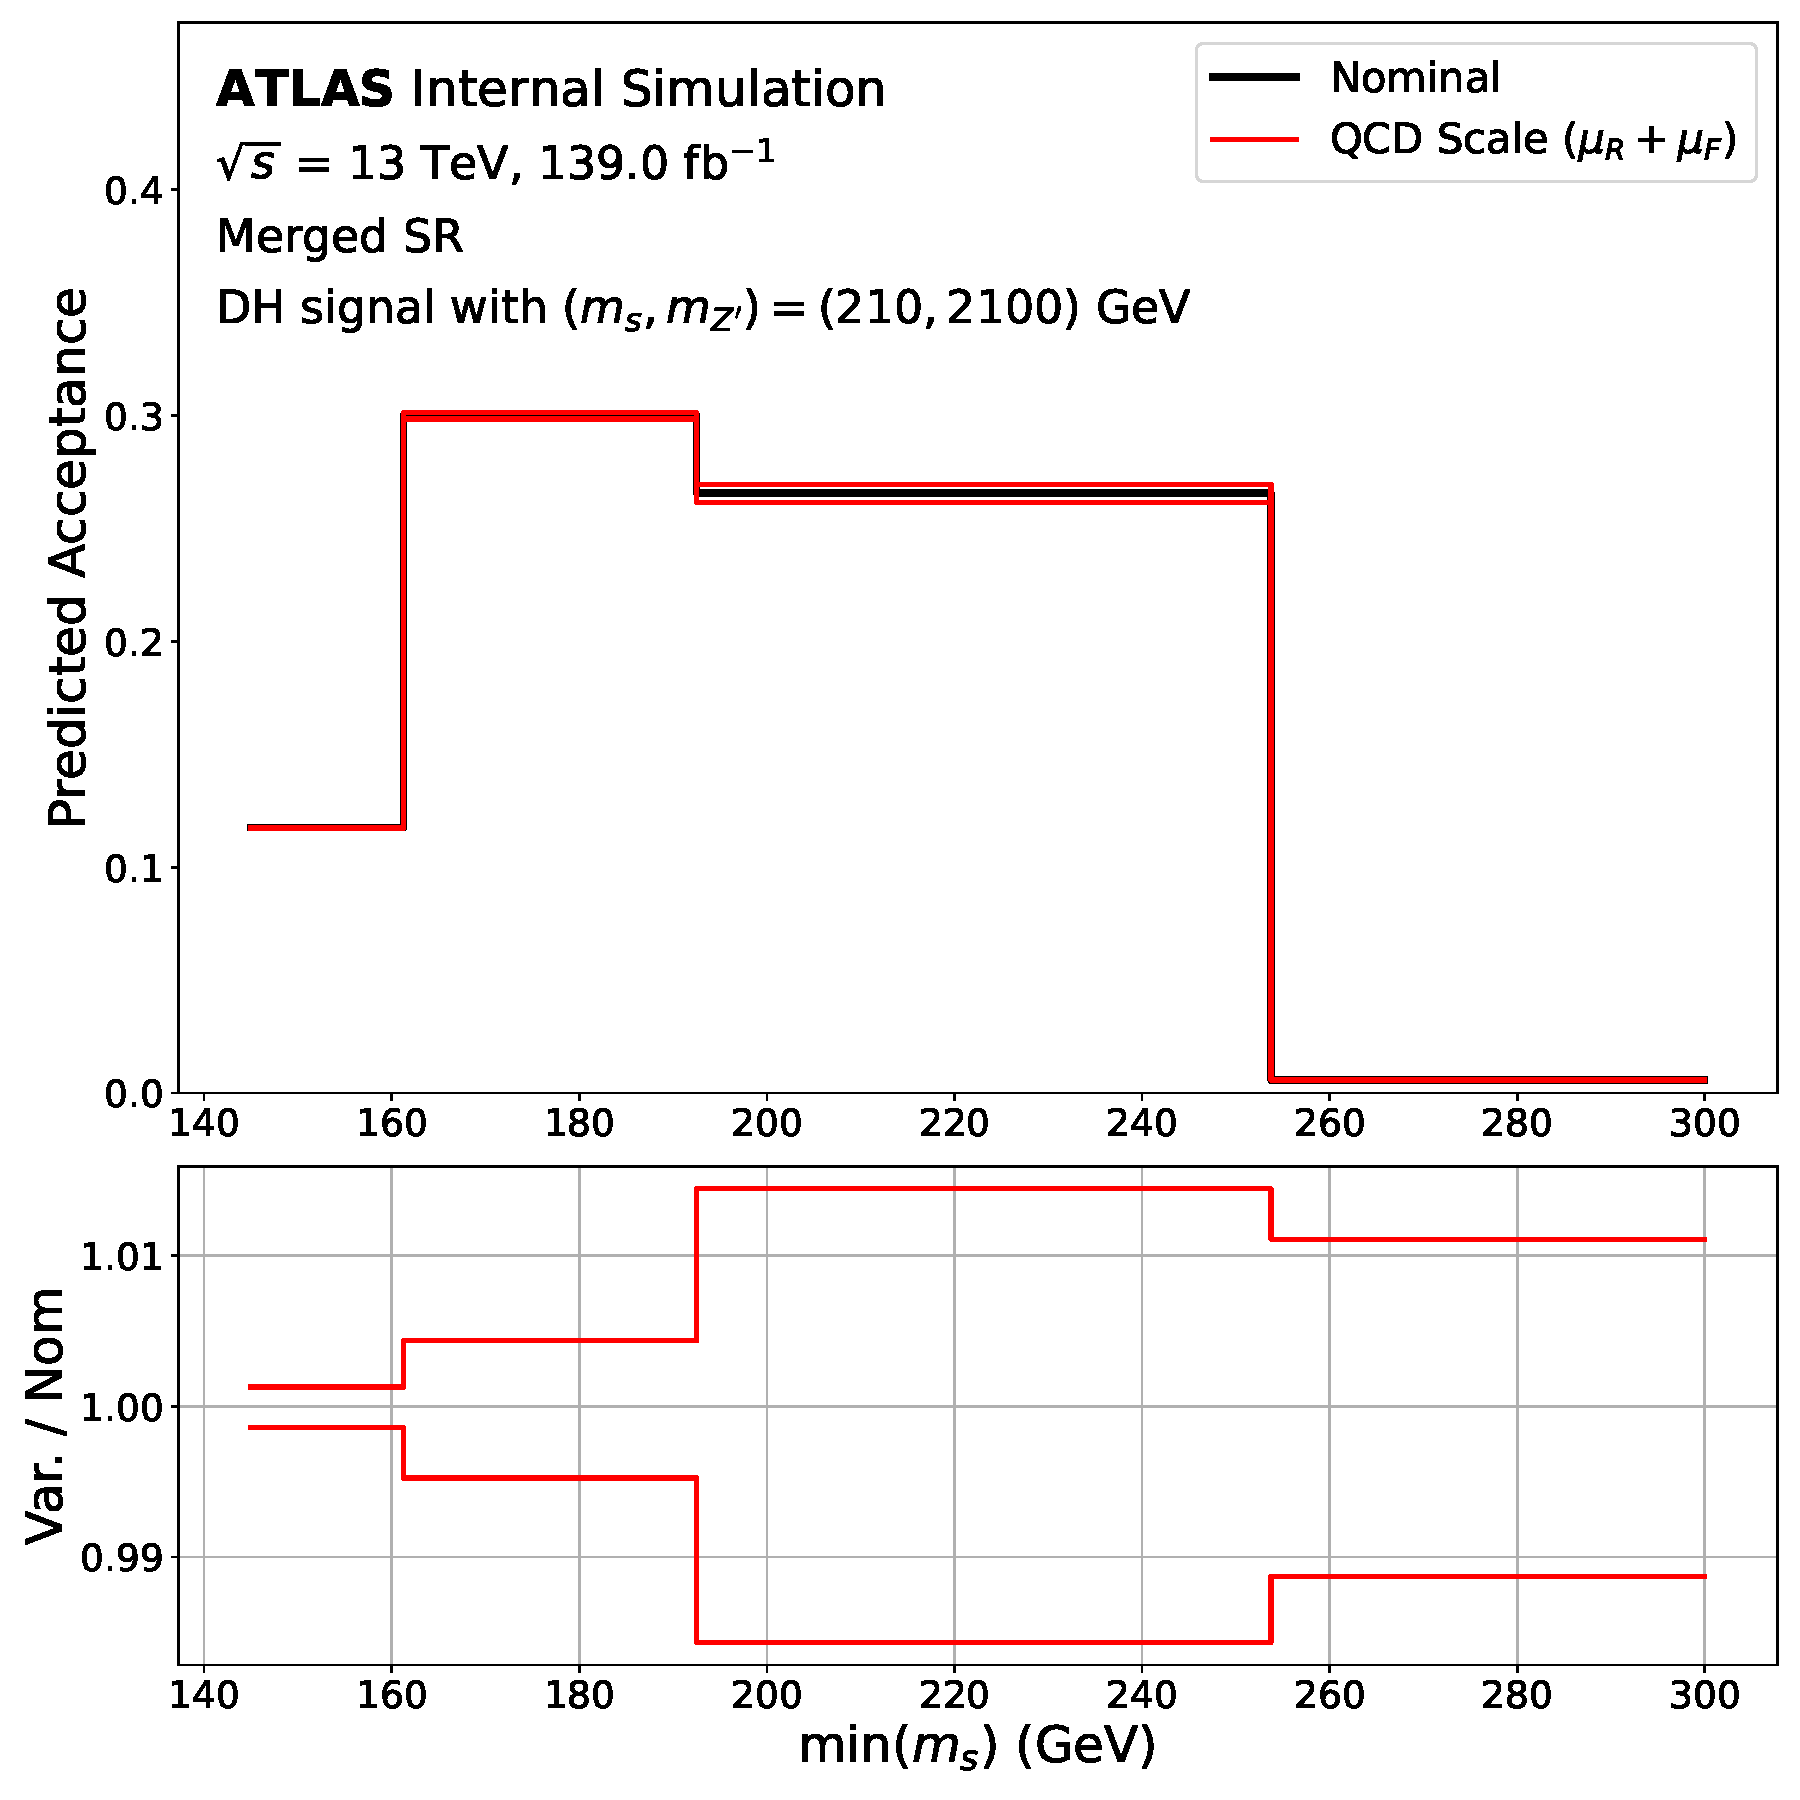
\includegraphics[width=0.9\textwidth]{Figures/6/scale_syst_monoSWWsemilep_zp2100_dm200_dh210_SR_mgd_TARJets10_minmS_mgd_symm_scale.pdf}
    \caption{\(\mu_R+\mu_F\) for DH signal at \((\ms, \mZp)=(210, 2100)~\GeV\)}
    \label{fig:DH_scale}
  \end{subfigure} \\ \vspace{1em}
      \caption{Shifts in the predicted yield of various processes considered in the search in the merged SRs due to theoretical systematic uncertainties. The predicted yield is binned in \minms using the binning strategy employed in the fit used to search for evidence of the DH signal model in the data (see Chapter \ref{chapter:stat} for details). Bottom panel shows ratio of the shifts relative to the nominal yield. }
  \label{fig:theory_systs}
  \end{figure}
  
 \begin{figure} \ContinuedFloat
  \begin{subfigure}{0.45\textwidth}
      \centering
    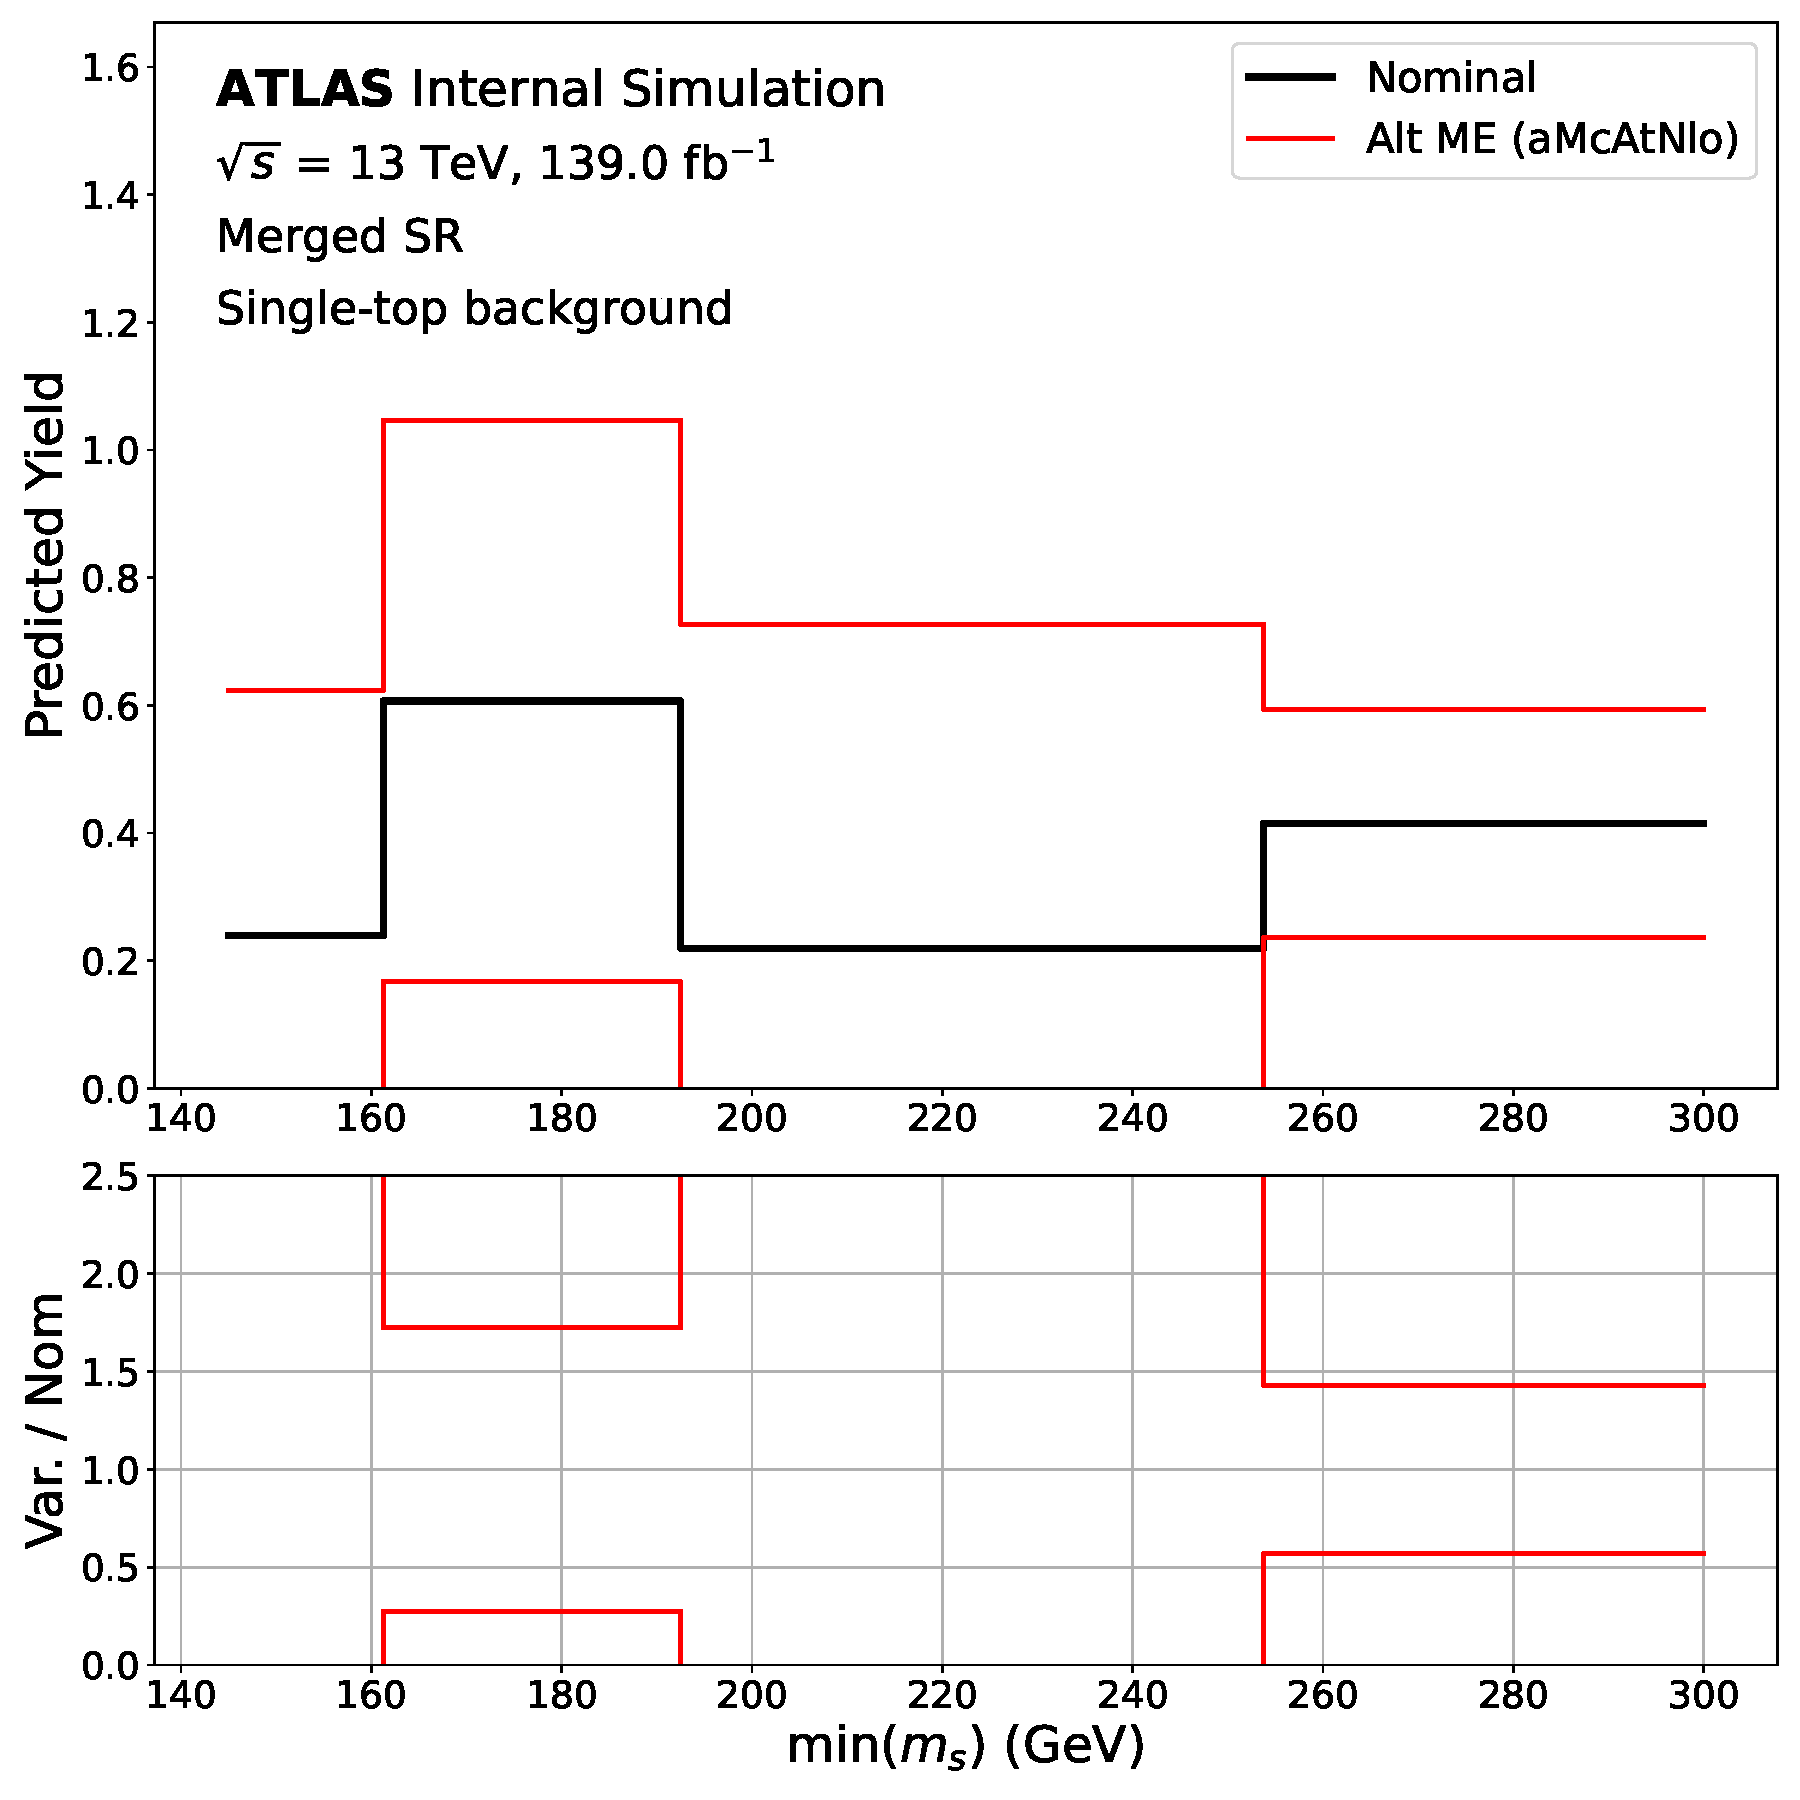
\includegraphics[width=0.9\textwidth]{Figures/6/2pt_AMcPy8_syst_stop_SR_mgd_TARJets10_minmS_mgd_yield.pdf}
    \caption{ME for single-top background}\label{fig:stop_ME}
    \end{subfigure} \hspace{1em}
   \begin{subfigure}{0.45\textwidth}
       \centering
    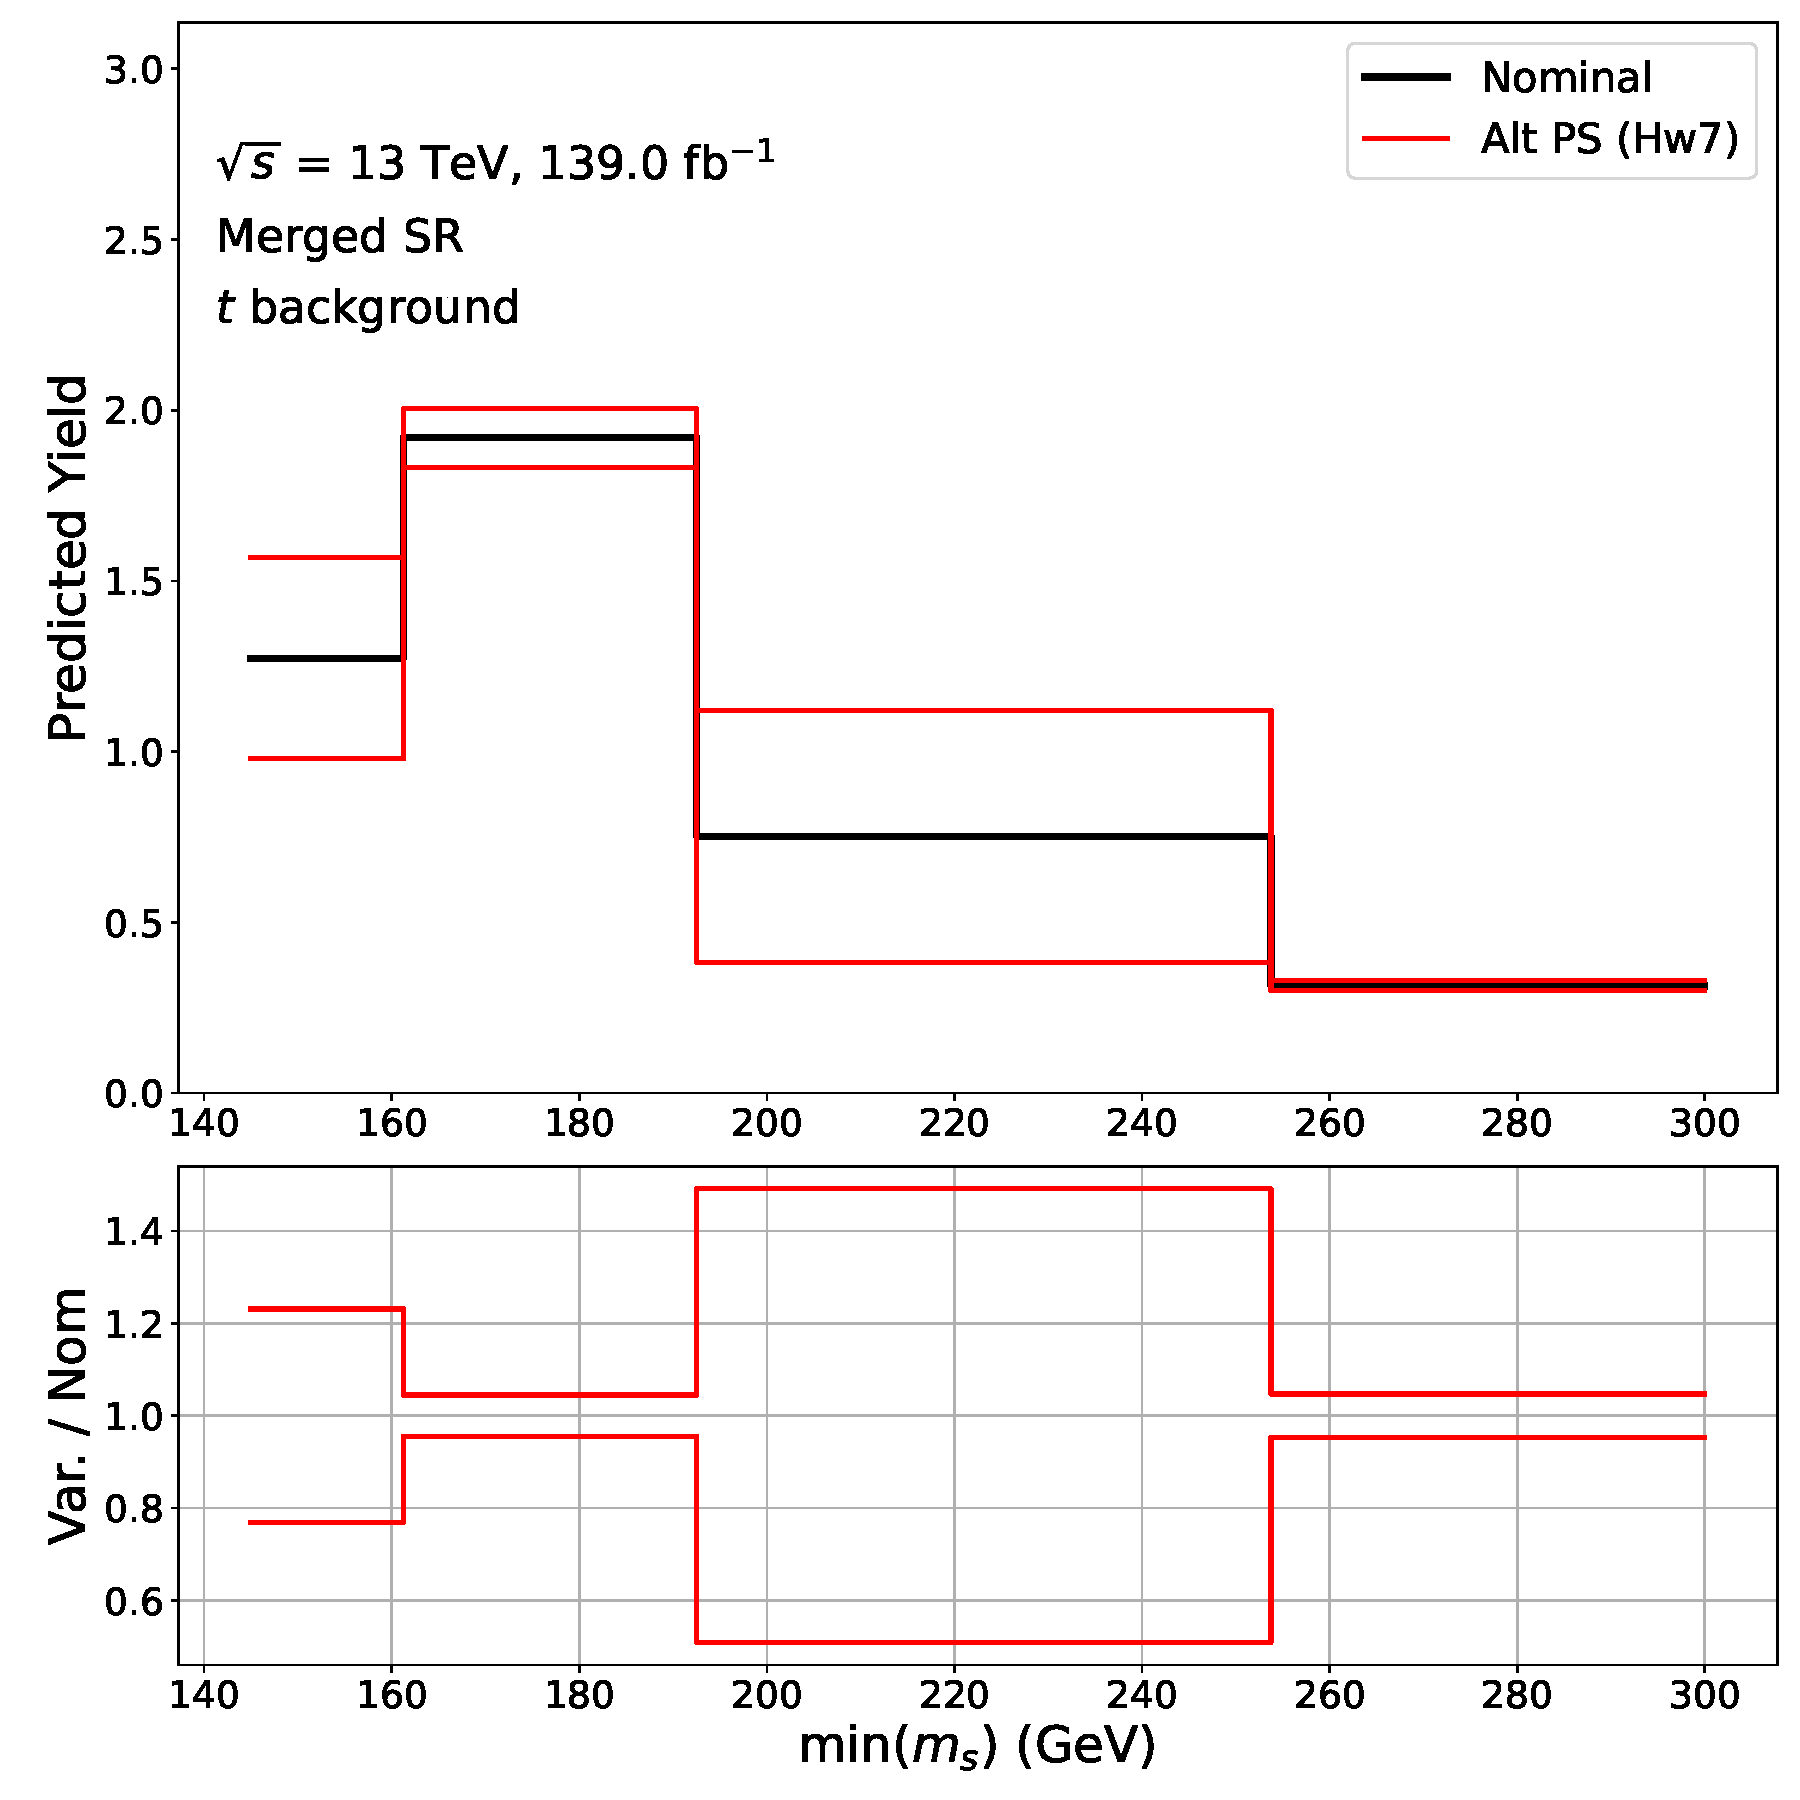
\includegraphics[width=0.9\textwidth]{Figures/6/2pt_PhHw7_syst_ttbar_SR_mgd_TARJets10_minmS_mgd_yield.pdf}
    \caption{PS for \ttbar background}\label{fig:ttbar_PS}
  \end{subfigure} \\ \vspace{1em}

  \begin{subfigure}{0.45\textwidth}
      \centering
    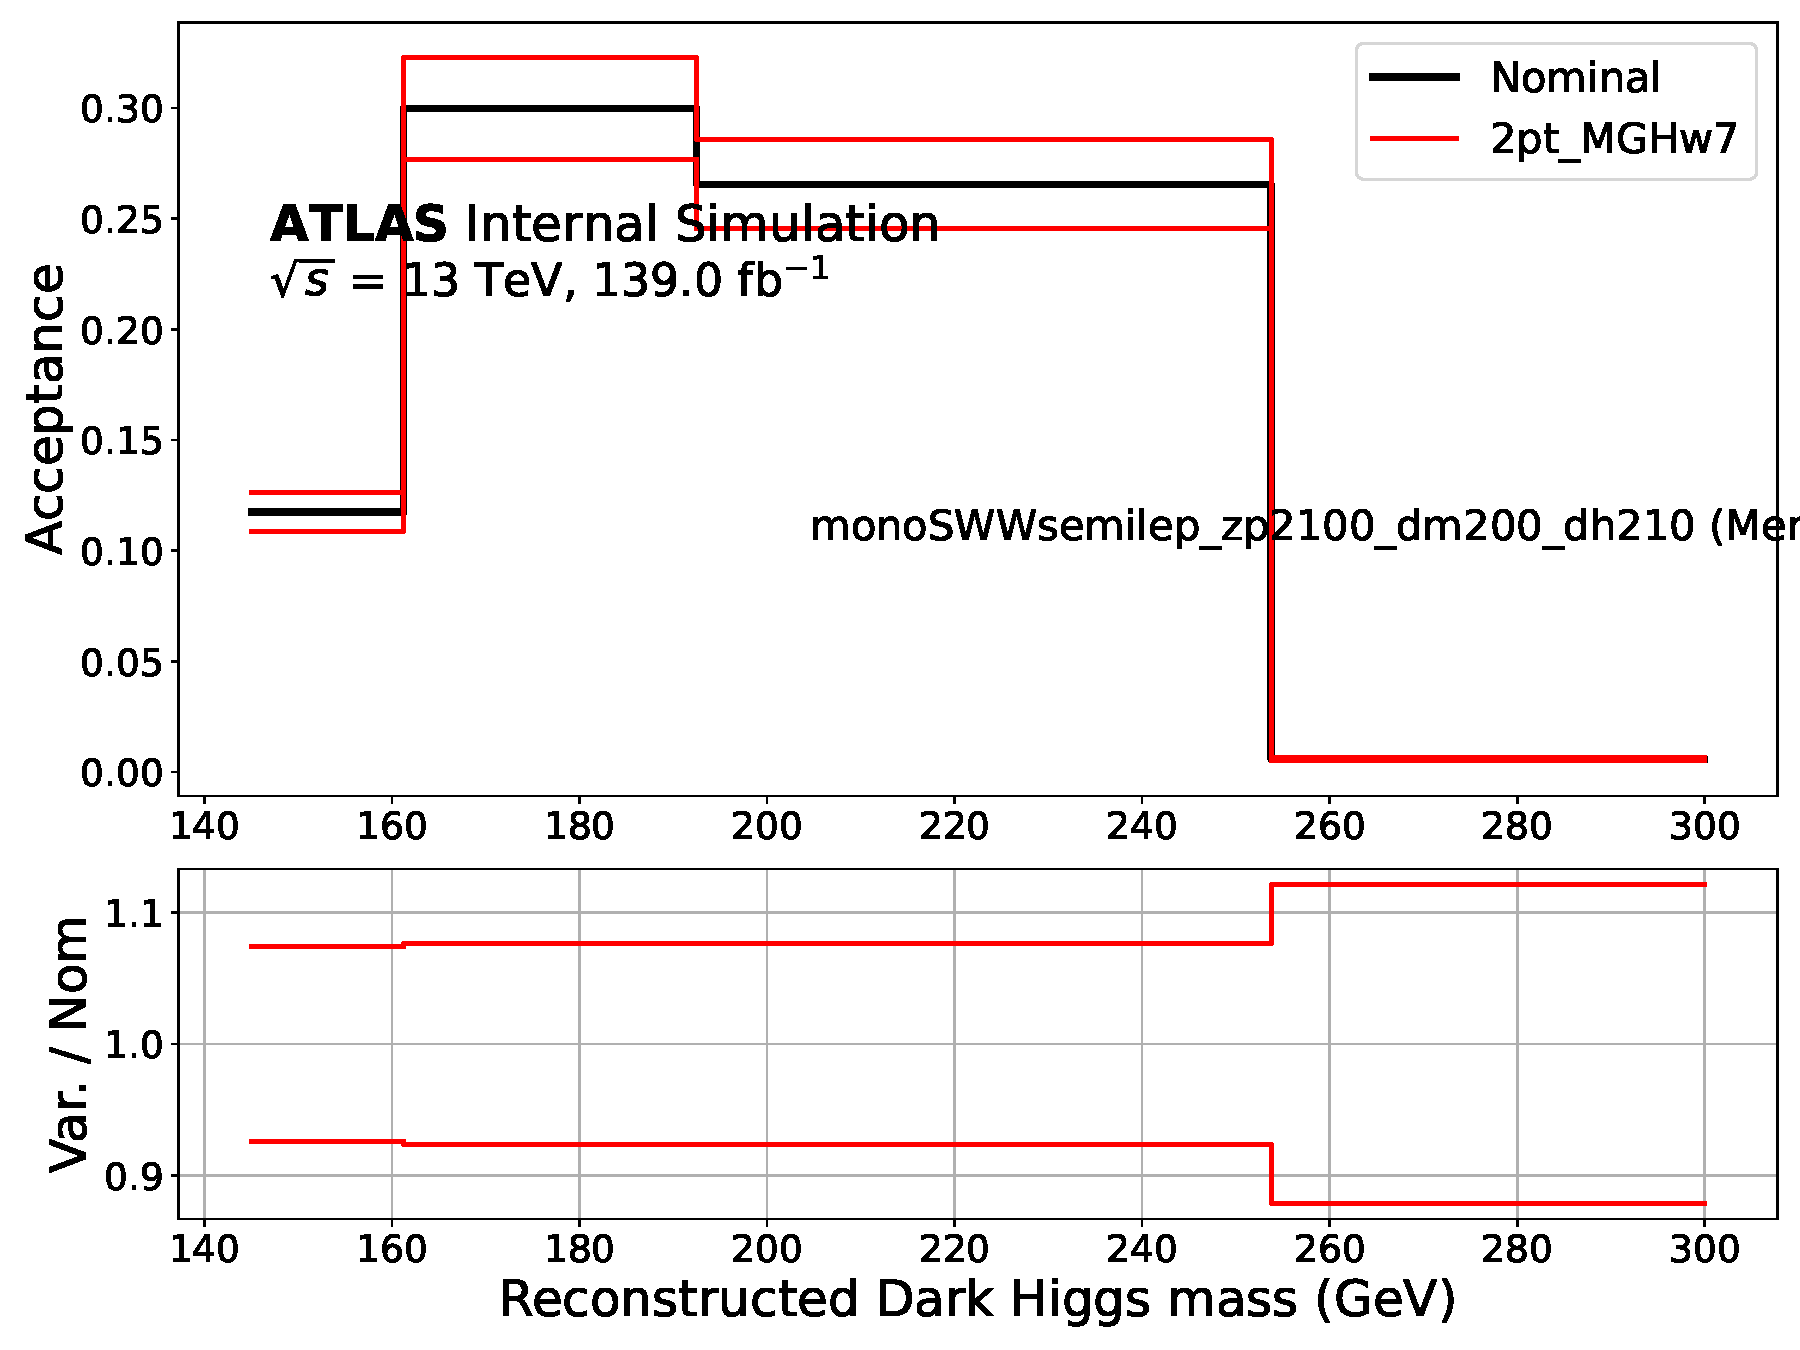
\includegraphics[width=0.9\textwidth]{Figures/6/2pt_MGHw7_syst_monoSWWsemilep_zp2100_dm200_dh210_SR_mgd_TARJets10_minmS_mgd.pdf}
    \caption{PS for DH signal at \((\ms, \mZp)=(210, 2100)~\GeV\)}
    \label{fig:DH_PS}
  \end{subfigure} \hspace{1em}
  \begin{subfigure}{0.45\textwidth}
      \centering
    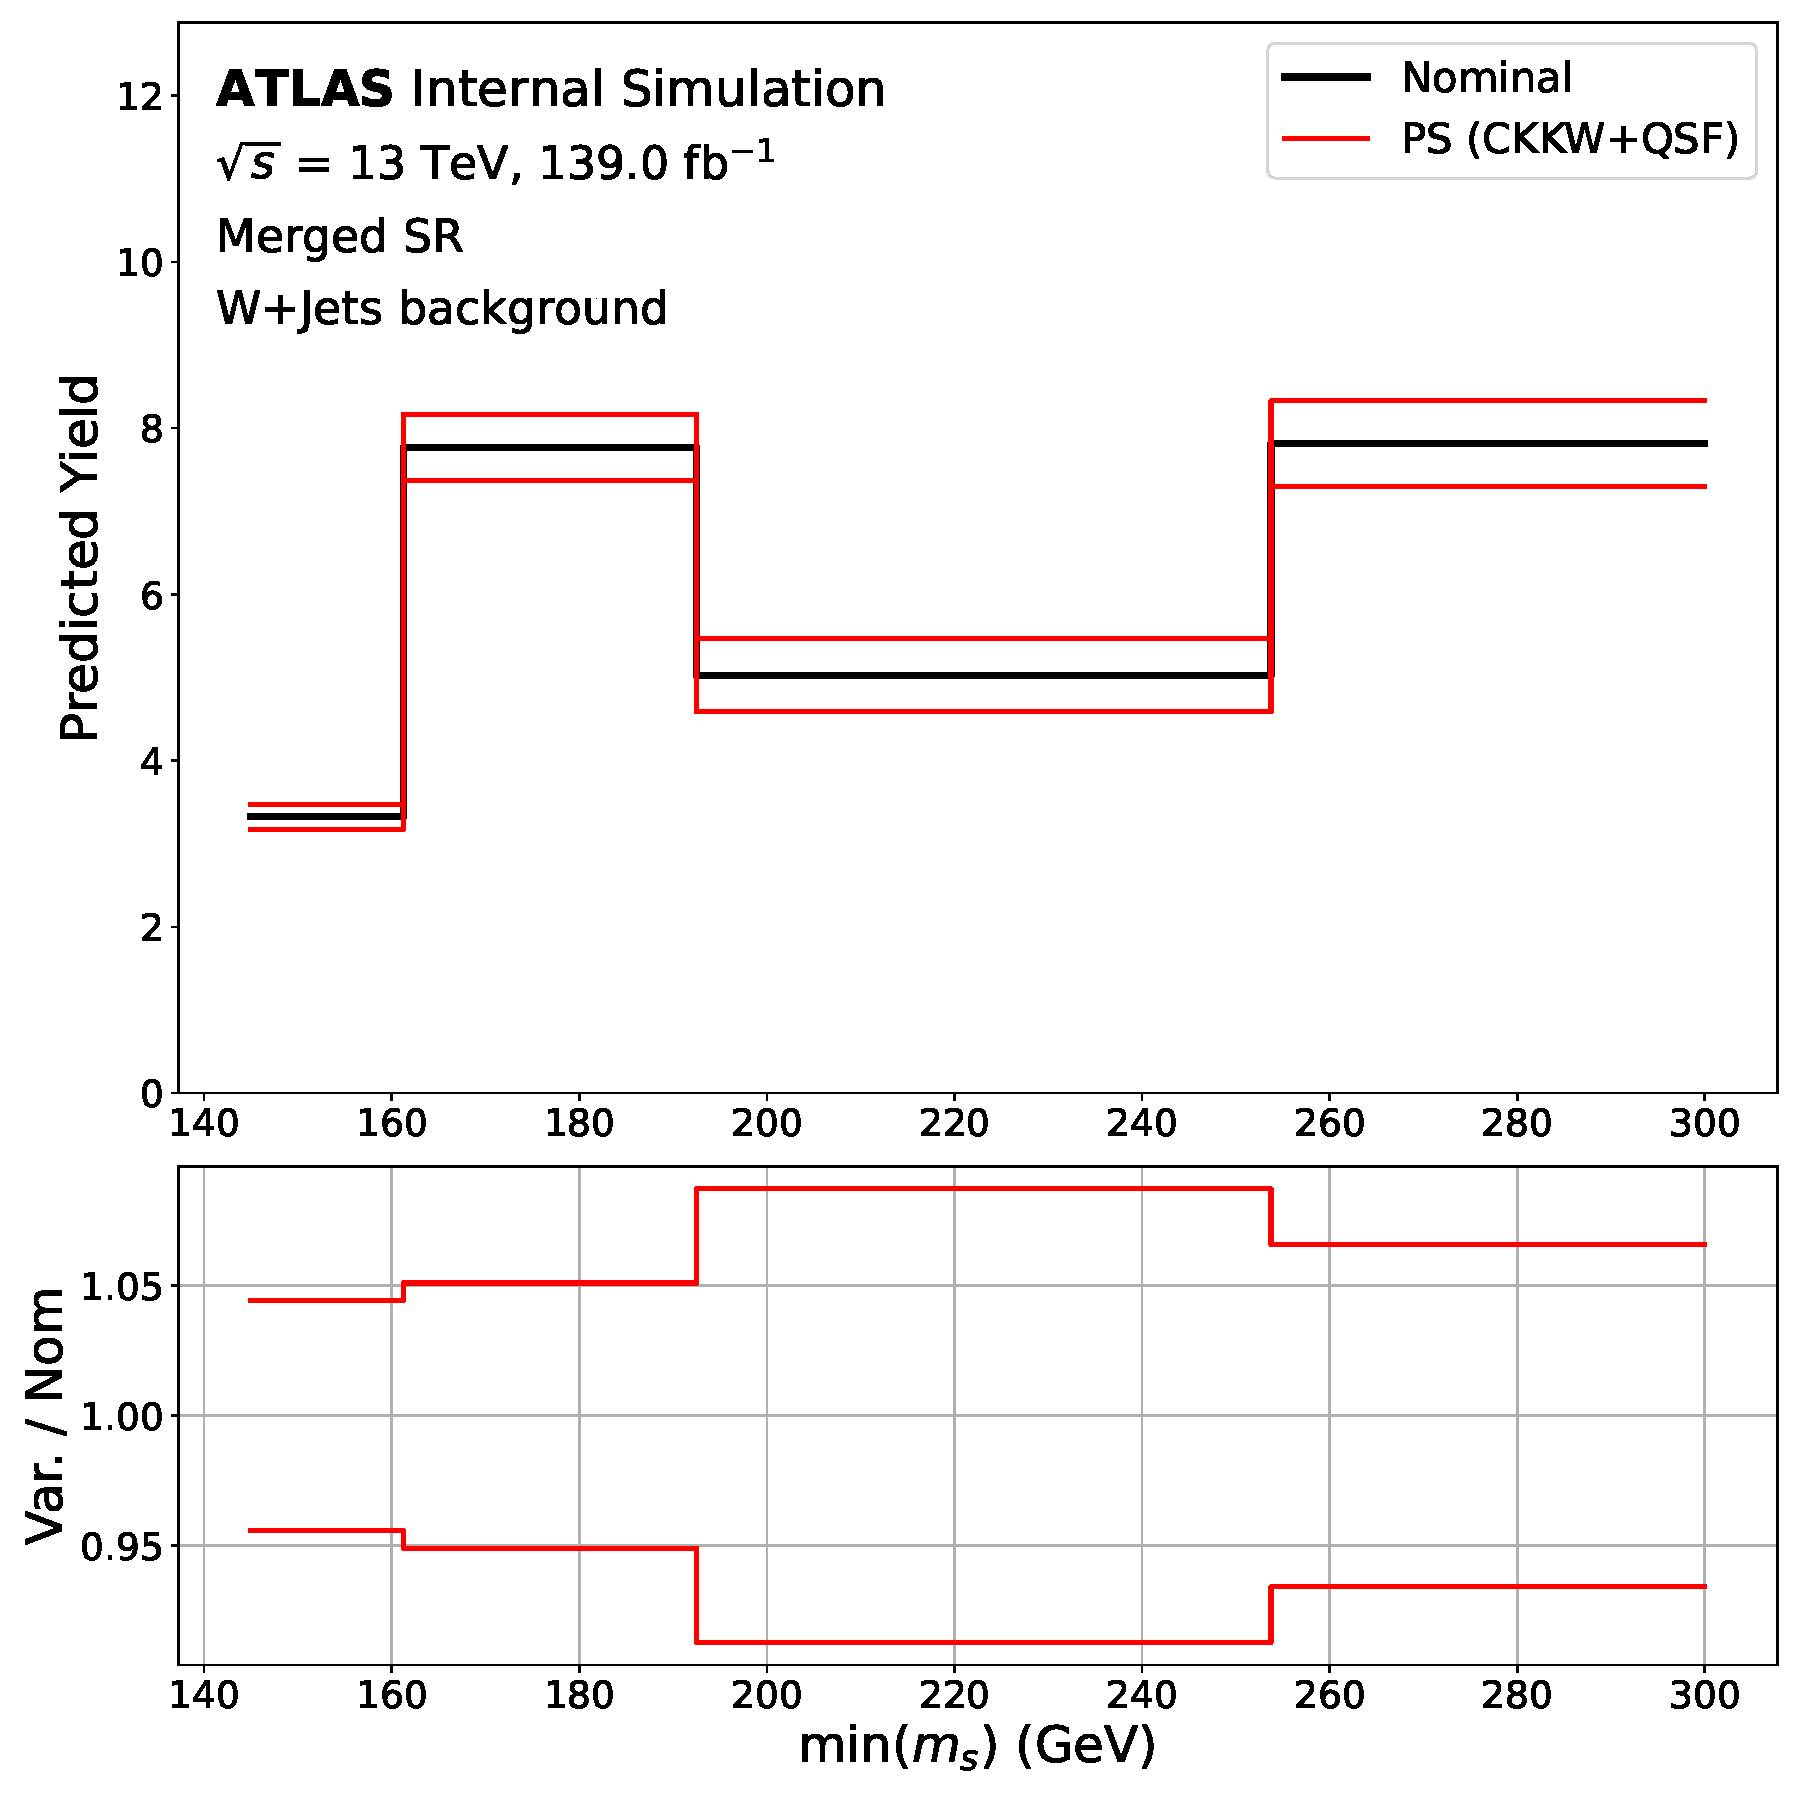
\includegraphics[width=0.9\textwidth]{Figures/6/ckkw_plus_qsf_syst_W+Jets_SR_mgd_TARJets10_minmS_mgd_yield.pdf}
    \caption{PS (CKKW+QSF) for \wjets background}
    \label{fig:wjets_PS}
  \end{subfigure} \\ \vspace{1em}
  
  \begin{subfigure}{0.45\textwidth}
      \centering
    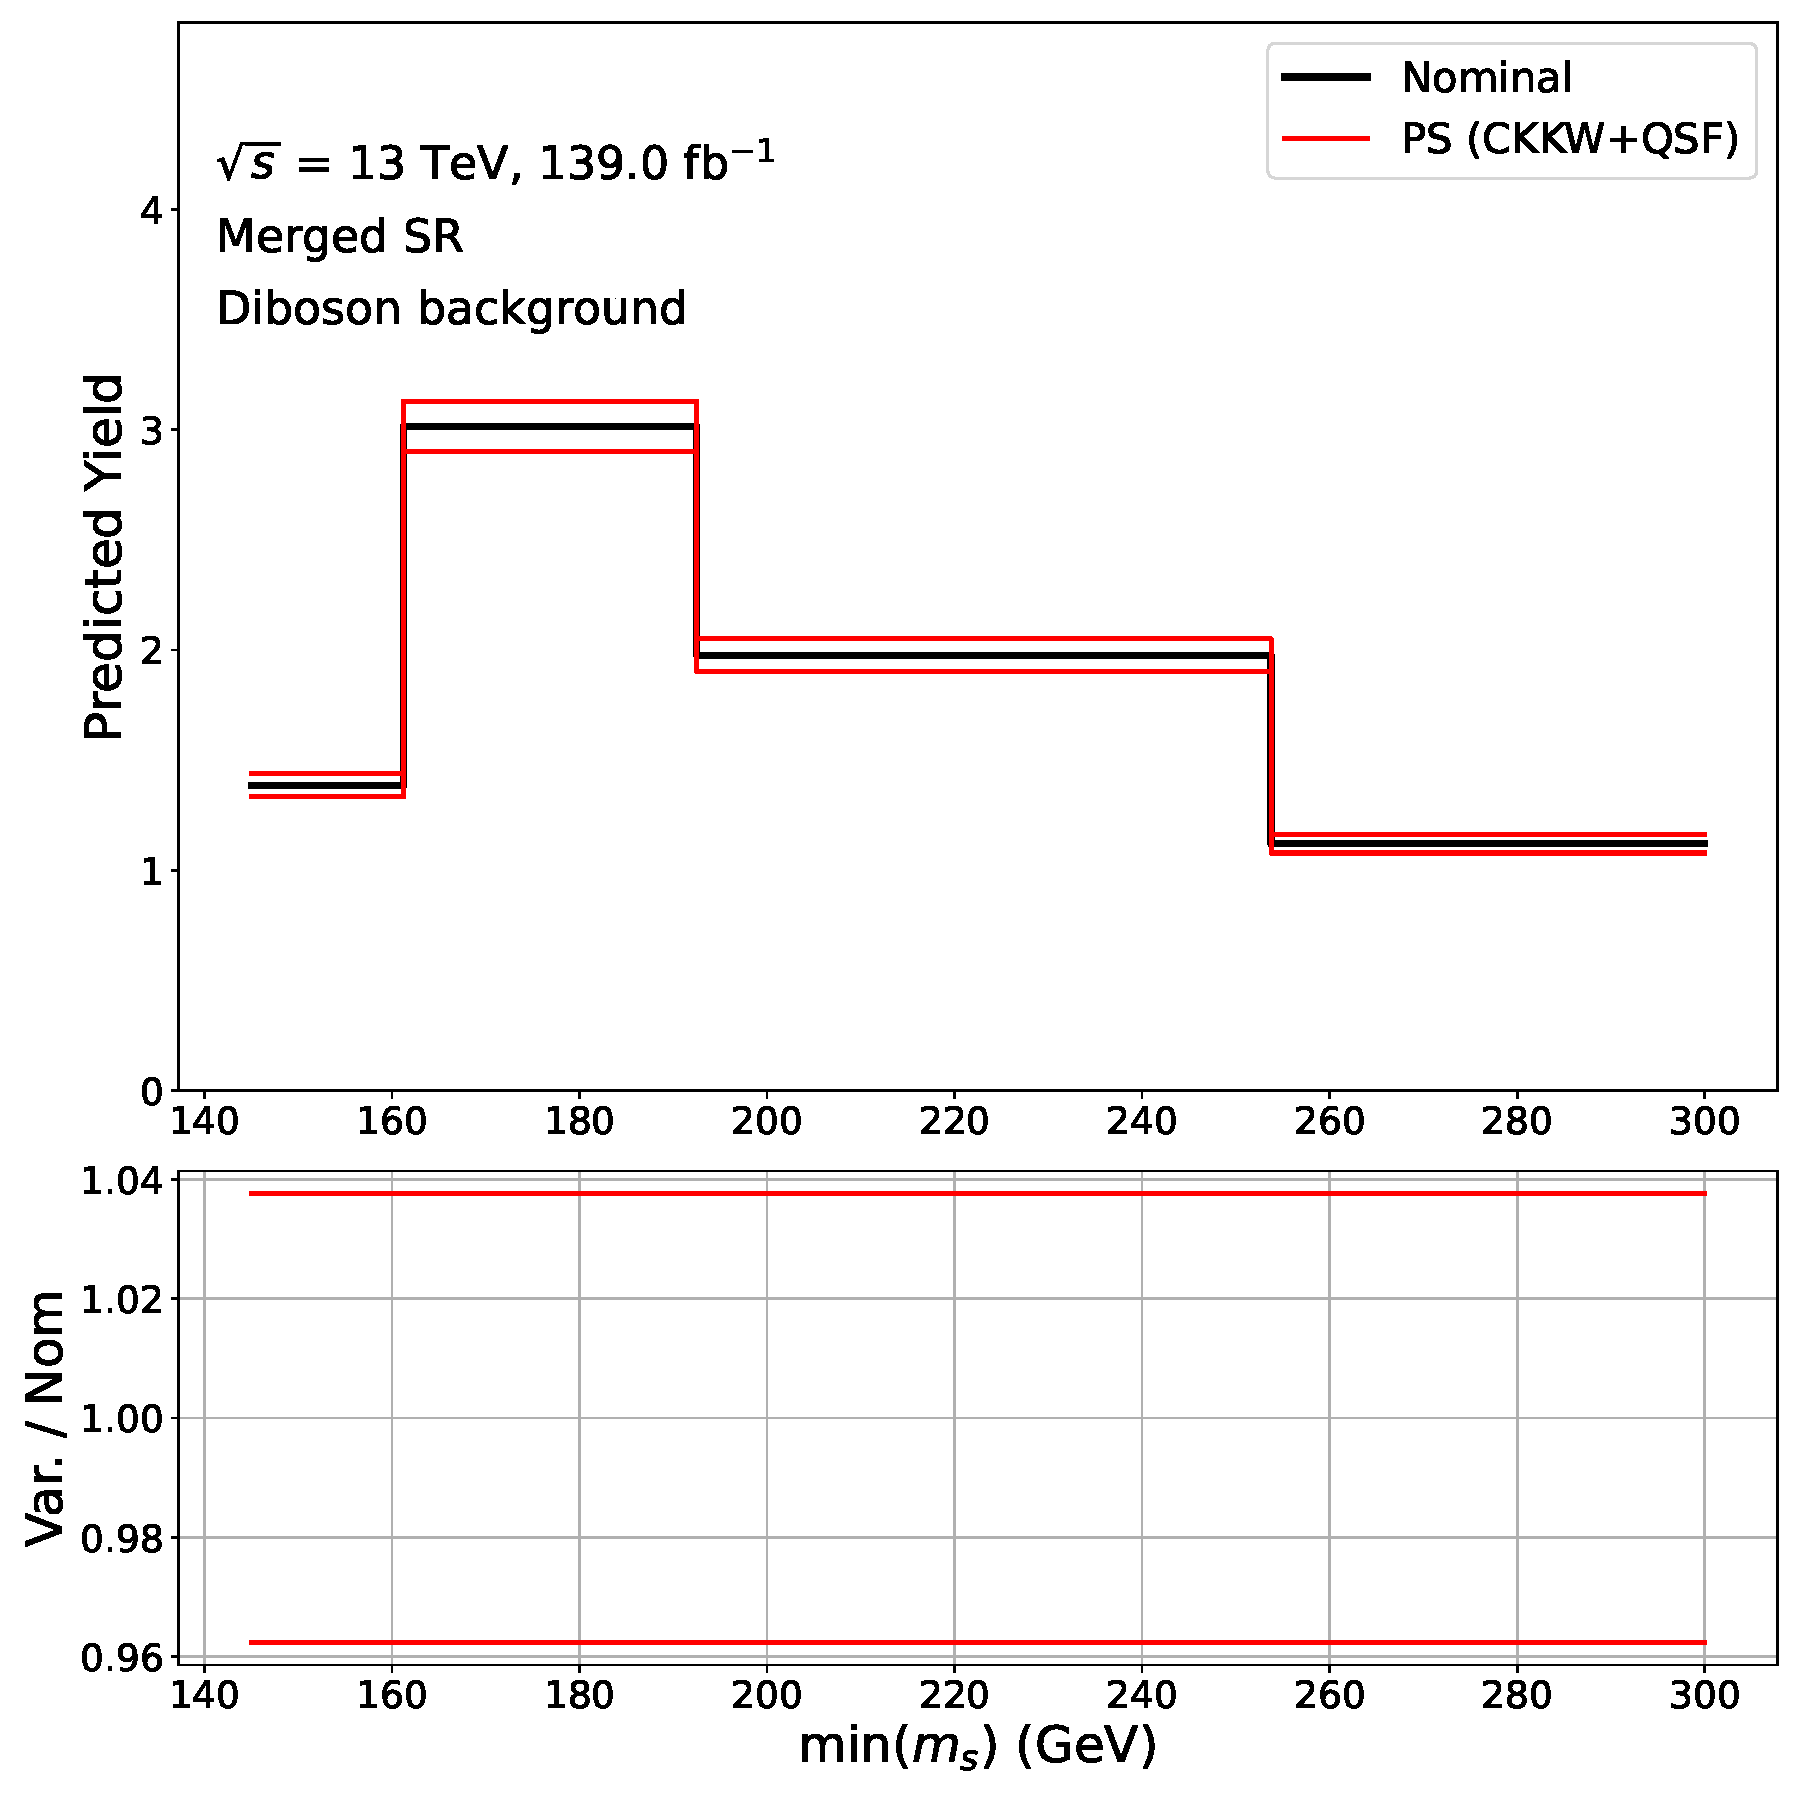
\includegraphics[width=0.9\textwidth]{Figures/6/ckkw_plus_qsf_syst_Diboson_SR_mgd_TARJets10_minmS_mgd_yield.pdf}
    \caption{PS (CKKW+QSF) for diboson background}
    \label{fig:diboson_PS}
  \end{subfigure} \hspace{1em}
  \begin{subfigure}{0.45\textwidth}
      \centering
    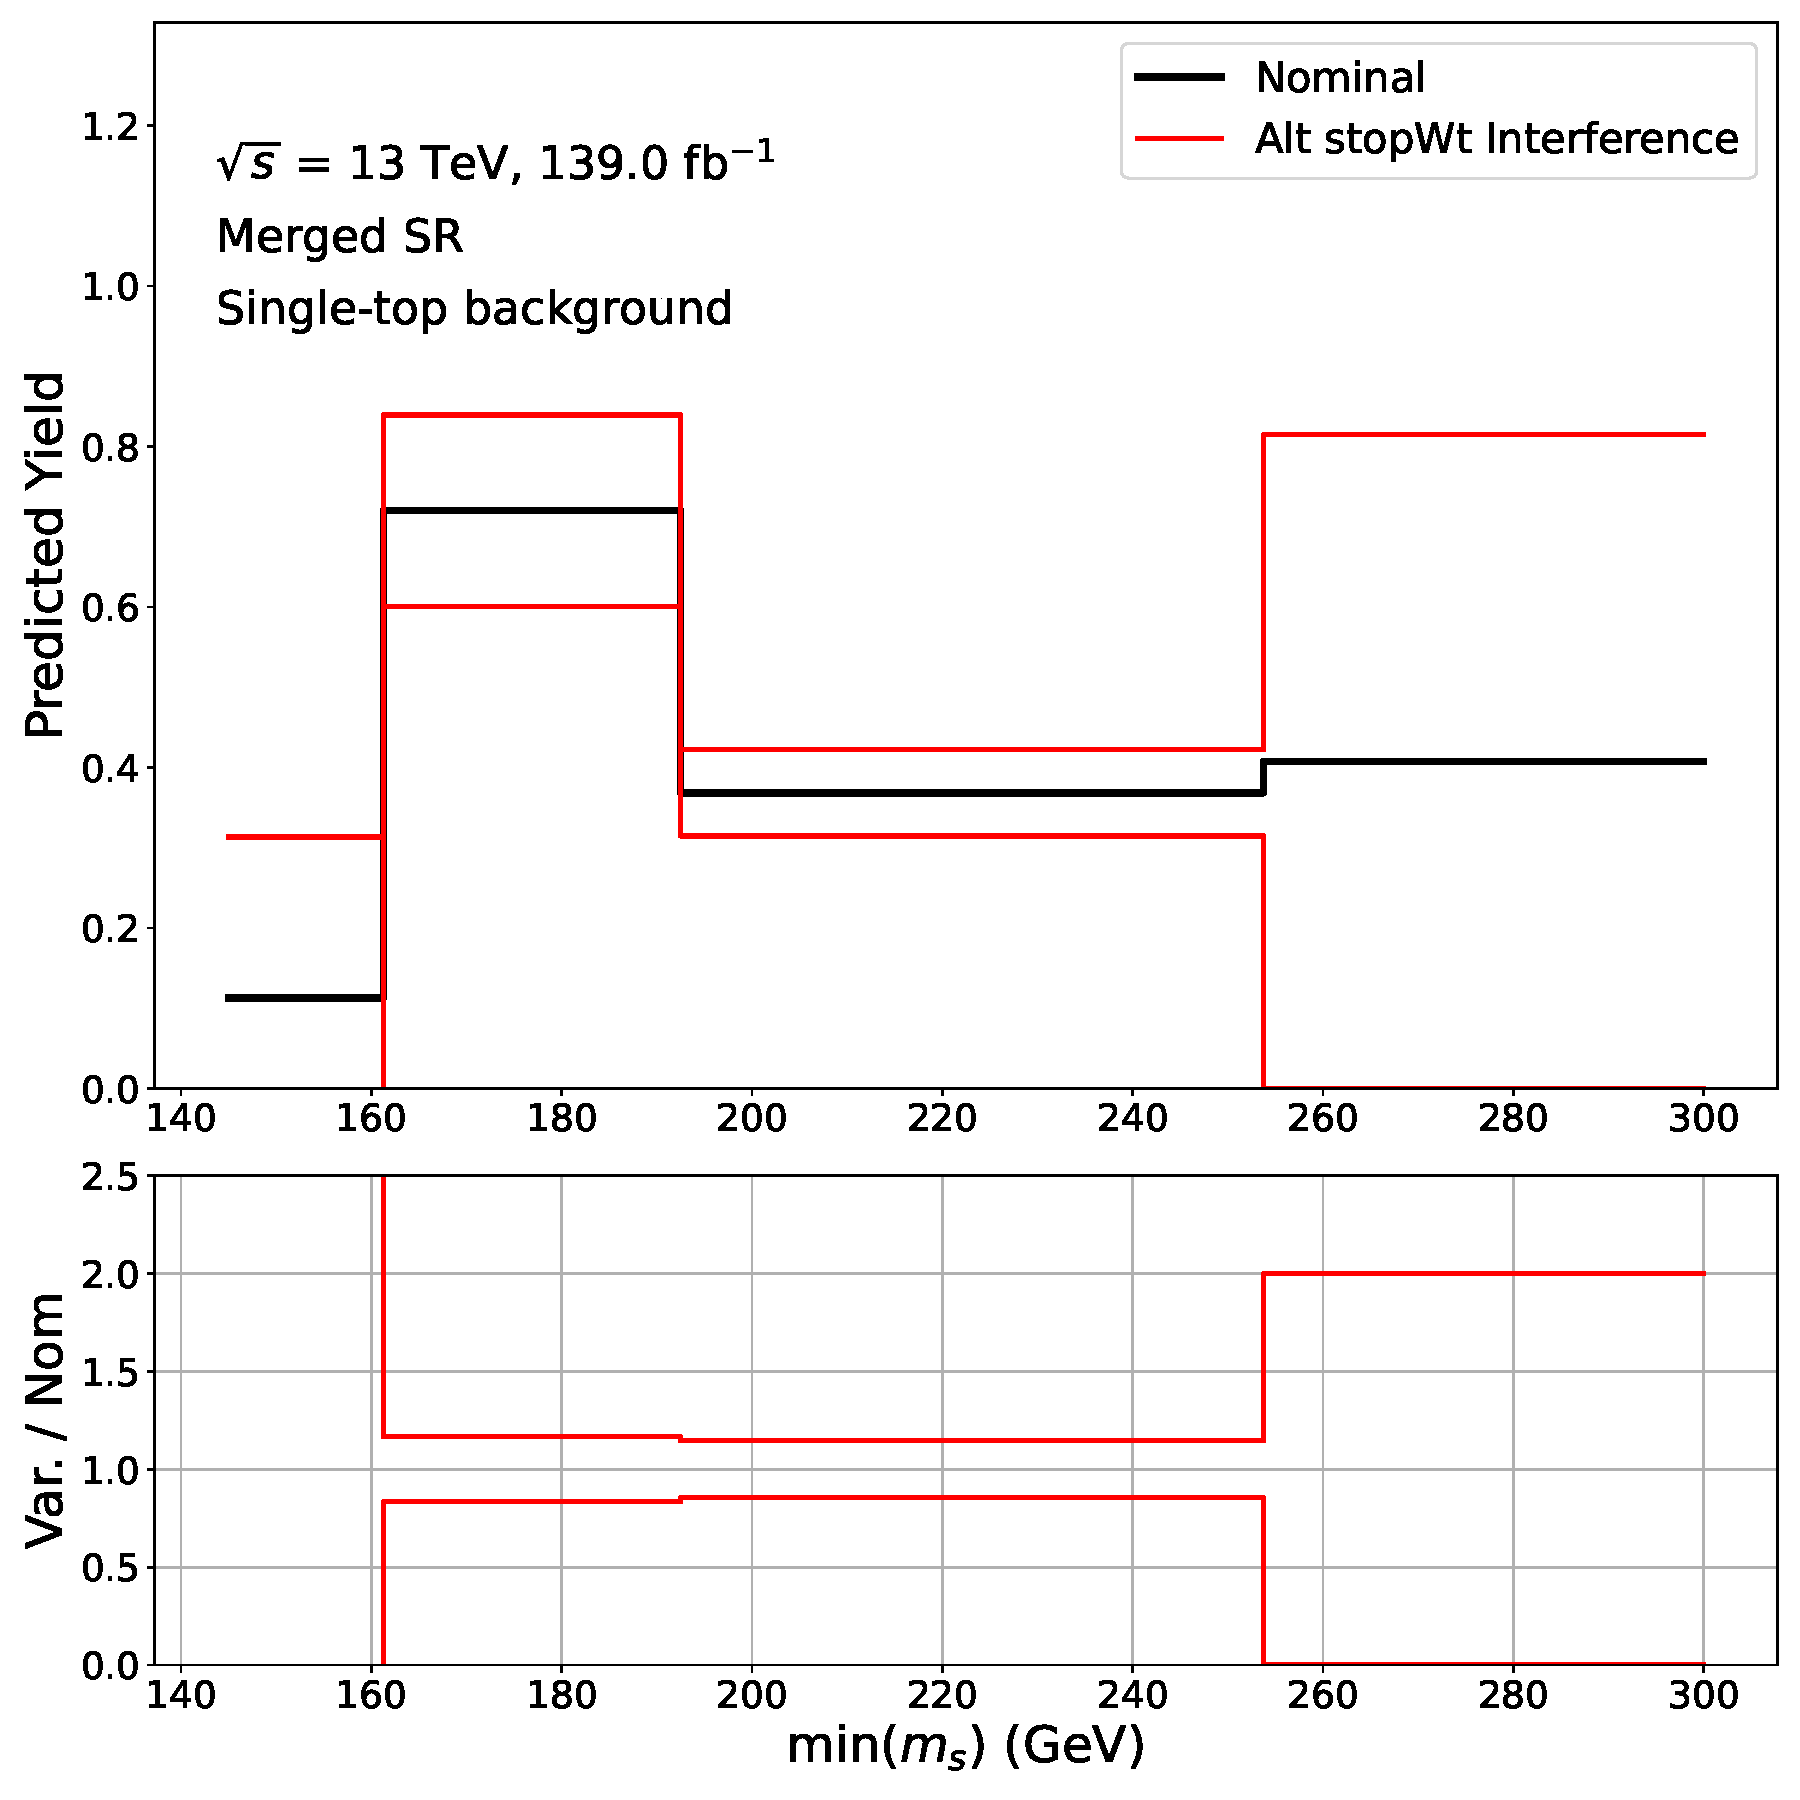
\includegraphics[width=0.9\textwidth]{Figures/6/2pt_DS_syst_stop_SR_mgd_TARJets10_minmS_mgd_yield.pdf}
    \caption{\(Wt\)/\ttbar Interference for single-top background}
    \label{fig:stop_DS}
  \end{subfigure}
  \caption{Shifts in the predicted yield due to theoretical systematic uncertainties (continued) }
\end{figure}

Tables \ref{tab:systs_bkg_SR} and \ref{tab:systs_bkg_CR} summarize the uncertainties associated with the total predicted yield from all theoretical sources for each background process in the SRs and CRs, respectively. 

\begin{table}[ht]
\small{
\caption{\label{tab:systs_bkg_SR} Theoretical systematic uncertainties associated with predicted yields of dominant backgrounds in the SRs, reported both in terms of absolute yield, and (in parentheses) as percent relative to nominal yield.}
\begin{tabular}{l l l l l l l }
\toprule
\textbf{Bkg and Syst.} & \textbf{Mgd SR} & \textbf{Res SR}\tabularnewline
\midrule
\midrule
W+Jets \(\mu_R\)+\(\mu_F\) & \(\substack{+6.33\\-3.14}\) \big(\(\substack{+26.45\%\\-13.12\%}\)\big) & \(\substack{+35.68\\-43.68}\) \big(\(\substack{+14.97\%\\-18.33\%}\)\big) \tabularnewline
\midrule
W+Jets PDF+\(\alpha_s\) & \(\pm\)1.08 (\(\pm\)4.53\%) & \(\pm\)3.27 (\(\pm\)1.37\%) \tabularnewline
\midrule
W+Jets PS & \(\pm\)1.25 (\(\pm\)6.22\%) & \(\pm\)16.31 (\(\pm\)7.54\%) \tabularnewline
\midrule
diboson \(\mu_R\)+\(\mu_F\) & \(\substack{+1.29\\-1.13}\) \big(\(\substack{+17.39\%\\-15.29\%}\)\big) & \(\substack{+7.62\\-6.60}\) \big(\(\substack{+15.22\%\\-13.19\%}\)\big) \tabularnewline
\midrule
diboson PDF+\(\alpha_s\) & \(\pm\)2.44 (\(\pm\)33.05\%) &\(\pm\)16.25 (\(\pm\)32.46\%) \tabularnewline
\midrule
diboson PS & \(\pm\)0.28 (\(\pm\)3.77\%) &\(\pm\)1.89 (\(\pm\)3.77\%) \tabularnewline
\midrule
\(t\bar{t}\) PS & \(\pm\)1.05 (\(\pm\)24.88\%) & \(\pm\)1.21 (\(\pm\)5.73\%) \tabularnewline
\midrule
\(t\bar{t}\) ME & \(\pm\)1.59 (\(\pm\)37.73\%) & \(\pm\)5.60 (\(\pm\)26.59\%) \tabularnewline
\midrule
\(t\bar{t}\) PDF & \(\pm\)0.03 (\(\pm\)0.78\%) & \(\pm\)0.09 (\(\pm\)0.42\%) \tabularnewline
\midrule
\(t\bar{t}\) \(\mu_R\)+\(\mu_F\) (ME) & \(\substack{+0.16\\-0.22}\) \big(\(\substack{+3.81\%\\-5.26\%}\)\big) & \(\substack{+0.58\\-0.85}\) \big(\(\substack{+2.74\%\\-4.02\%}\)\big) \tabularnewline
\midrule
\(t\bar{t}\) ISR \(\alpha_s\) & \(\pm\)0.04 (\(\pm\)0.95\%) & \(\pm\)0.24 (\(\pm\)1.12\%) \tabularnewline
\midrule
\(t\bar{t}\) \(\mu_R\) (FSR) & \(\pm\)0.46 (\(\pm\)10.87\%) & \(\pm\)0.67 (\(\pm\)3.19\%) \tabularnewline
\midrule
stop PS & \(\pm\)0.72 (\(\pm\)48.73\%) &\(\pm\)3.00 (\(\pm\)79.77\%) \tabularnewline
\midrule
stop ME & \(\pm\)1.51 (\(\pm\)101.97\%) &\(\pm\)2.74 (\(\pm\)72.92\%) \tabularnewline
\midrule
stop \(Wt\)/\ttbar & \(\pm\)0.82 (\(\pm\)55.18\%) &\(\pm\)2.35 (\(\pm\)62.38\%) \tabularnewline
\midrule
stop PDF & \(\pm\)0.06 (\(\pm\)3.87\%) &\(\pm\)0.08 (\(\pm\)2.11\%) \tabularnewline
\midrule
stop \(\mu_R\)+\(\mu_F\) (ME) & \(\substack{+0.21\\-0.15}\) \big(\(\substack{+14.48\%\\-10.44\%}\)\big) & \(\substack{+0.38\\-0.28}\) \big(\(\substack{+10.09\%\\-7.41\%}\)\big) \tabularnewline
\midrule
stop ISR \(\alpha_s\) & \(\pm\)0.11 (\(\pm\)7.75\%) &\(\pm\)0.32 (\(\pm\)8.63\%) \tabularnewline
\midrule
stop \(\mu_R\) (FSR) & \(\pm\)1.21 (\(\pm\)81.86\%) &\(\pm\)1.57 (\(\pm\)41.61\%) \tabularnewline
\midrule
triboson \(\mu_R\)+\(\mu_F\) & \(\substack{+0.04\\-0.04}\) \big(\(\substack{+3.71\%\\-3.22\%}\)\big) & \(\substack{+0.12\\-0.10}\) \big(\(\substack{+4.29\%\\-3.75\%}\)\big) \tabularnewline
\midrule
triboson PDF+\(\alpha_s\) & \(\pm\)0.02 (\(\pm\)1.82\%) &\(\pm\)0.04 (\(\pm\)1.37\%) \tabularnewline
\midrule
triboson PS & \(\pm\)0.07 (\(\pm\)6.22\%) &\(\pm\)0.21 (\(\pm\)7.54\%) \tabularnewline
\midrule
Z+Jets \(\mu_R\)+\(\mu_F\) & \(\substack{+0.30\\-0.15}\) \big(\(\substack{+26.45\%\\-13.12\%}\)\big) & \(\substack{+2.59\\-3.17}\) \big(\(\substack{+14.97\%\\-18.33\%}\)\big) \tabularnewline
\midrule
Z+Jets PDF+\(\alpha_s\) & \(\pm\)0.05 (\(\pm\)4.53\%) &\(\pm\)0.24 (\(\pm\)1.37\%) \tabularnewline
\midrule
Z+Jets PS & \(\pm\)0.07 (\(\pm\)6.22\%) &\(\pm\)1.30 (\(\pm\)7.54\%) \tabularnewline
\bottomrule
\end{tabular}}
\end{table}

\begin{table}[ht]
\footnotesize{
\caption{\label{tab:systs_bkg_CR} Theoretical systematic uncertainties associated with predicted yields of dominant backgrounds in the CRs, reported both in terms of absolute yield, and (in parentheses) as percent relative to nominal yield.}
\begin{tabular}{l l l l l l l }
\toprule
\textbf{Bkg and Syst.} & \textbf{Mgd CRW} & \textbf{Res CRW} & \textbf{Mgd CRTT} & \textbf{Res CRTT}\tabularnewline
\midrule
\midrule
W+Jets \(\mu_R\)+\(\mu_F\) & \(\substack{+42.91\\-25.22}\) \big(\(\substack{+24.86\%\\-14.61\%}\)\big) & \(\substack{+36.17\\-61.14}\) \big(\(\substack{+6.08\%\\-10.28\%}\)\big) & \(\substack{+3.55\\-0.48}\) \big(\(\substack{+137.61\%\\-18.72\%}\)\big) & \(\substack{+6.27\\-0.93}\) \big(\(\substack{-262.80\%\\+39.21\%}\)\big) \tabularnewline
\midrule
W+Jets PDF+\(\alpha_s\) & \(\pm\)3.70 (\(\pm\)2.14\%) &\(\pm\)13.10 (\(\pm\)2.20\%) &\(\pm\)0.40 (\(\pm\)15.39\%) &\(\pm\)0.34 (\(\pm\)14.36\%) \tabularnewline
\midrule
W+Jets PS & \(\pm\)12.17 (\(\pm\)8.02\%) &\(\pm\)35.66 (\(\pm\)6.86\%) &\(\pm\)0.19 (\(\pm\)8.44\%) &\(\pm\)0.18 (\(\pm\)10.77\%) \tabularnewline
\midrule
diboson \(\mu_R\)+\(\mu_F\) & \(\substack{+1.02\\-4.14}\) \big(\(\substack{+3.84\%\\-15.64\%}\)\big) & \(\substack{+18.40\\-15.47}\) \big(\(\substack{+17.40\%\\-14.64\%}\)\big) & \(\substack{+0.04\\-0.03}\) \big(\(\substack{+19.96\%\\-15.00\%}\)\big) & \(\substack{+0.13\\-0.10}\) \big(\(\substack{+22.85\%\\-16.89\%}\)\big) \tabularnewline
\midrule
diboson PDF+\(\alpha_s\) & \(\pm\)8.75 (\(\pm\)33.11\%) &\(\pm\)33.29 (\(\pm\)31.48\%) &\(\pm\)0.05 (\(\pm\)21.92\%) &\(\pm\)0.17 (\(\pm\)29.03\%) \tabularnewline
\midrule
diboson PS & \(\pm\)1.00 (\(\pm\)3.77\%) &\(\pm\)3.99 (\(\pm\)3.77\%) &\(\pm\)0.00 &\(\pm\)0.02 (\(\pm\)3.77\%) \tabularnewline
\midrule
\(t\bar{t}\) PS & \(\pm\)0.75 (\(\pm\)7.72\%) &\(\pm\)1.94 (\(\pm\)9.82\%) &\(\pm\)11.39 (\(\pm\)16.13\%) &\(\pm\)12.01 (\(\pm\)18.71\%) \tabularnewline
\midrule
\(t\bar{t}\) ME & \(\pm\)3.57 (\(\pm\)36.93\%) &\(\pm\)0.27 (\(\pm\)1.35\%) &\(\pm\)1.84 (\(\pm\)2.60\%) &\(\pm\)8.77 (\(\pm\)13.67\%) \tabularnewline
\midrule
\(t\bar{t}\) PDF & \(\pm\)0.03 (\(\pm\)0.32\%) &\(\pm\)0.06 (\(\pm\)0.31\%) &\(\pm\)0.29 (\(\pm\)0.41\%) &\(\pm\)0.14 (\(\pm\)0.22\%) \tabularnewline
\midrule
\(t\bar{t}\) \(\mu_R\)+\(\mu_F\) (ME) & \(\substack{+0.35\\-0.25}\) \big(\(\substack{+3.61\%\\-2.63\%}\)\big) & \(\substack{+1.26\\-0.87}\) \big(\(\substack{+6.37\%\\-4.39\%}\)\big) & \(\substack{+2.46\\-3.82}\) \big(\(\substack{+3.48\%\\-5.40\%}\)\big) & \(\substack{+1.04\\-1.66}\) \big(\(\substack{+1.62\%\\-2.58\%}\)\big) \tabularnewline
\midrule
\(t\bar{t}\) ISR \(\alpha_s\) & \(\pm\)0.01 (\(\pm\)0.14\%) &\(\pm\)0.11 (\(\pm\)0.57\%) &\(\pm\)0.72 (\(\pm\)1.02\%) &\(\pm\)0.04 (\(\pm\)0.06\%) \tabularnewline
\midrule
\(t\bar{t}\) \(\mu_R\)+\(\mu_F\) (FSR) & \(\pm\)1.15 (\(\pm\)11.89\%) &\(\pm\)0.61 (\(\pm\)3.10\%) &\(\pm\)5.27 (\(\pm\)7.46\%) &\(\pm\)2.88 (\(\pm\)4.49\%) \tabularnewline
\midrule
stop PS & \(\pm\)2.51 (\(\pm\)80.16\%) &\(\pm\)1.09 (\(\pm\)33.41\%) &\(\pm\)2.09 (\(\pm\)37.87\%) &\(\pm\)4.49 (\(\pm\)41.21\%) \tabularnewline
\midrule
stop ME & \(\pm\)0.02 (\(\pm\)0.73\%) &\(\pm\)1.68 (\(\pm\)51.31\%) &\(\pm\)1.62 (\(\pm\)29.40\%) &\(\pm\)1.97 (\(\pm\)18.07\%) \tabularnewline
\midrule
stop \(Wt\)/\ttbar & \(\pm\)3.47 (\(\pm\)110.52\%) &\(\pm\)1.18 (\(\pm\)35.96\%) &\(\pm\)3.95 (\(\pm\)71.68\%) &\(\pm\)7.81 (\(\pm\)71.75\%) \tabularnewline
\midrule
stop PDF & \(\pm\)0.12 (\(\pm\)3.67\%) &\(\pm\)0.17 (\(\pm\)5.16\%) &\(\pm\)0.11 (\(\pm\)1.94\%) &\(\pm\)0.28 (\(\pm\)2.58\%) \tabularnewline
\midrule
stop \(\mu_R\)+\(\mu_F\) (ME) & \(\substack{+0.59\\-0.39}\) \big(\(\substack{+18.89\%\\-12.45\%}\)\big) & \(\substack{+0.46\\-0.34}\) \big(\(\substack{+14.03\%\\-10.46\%}\)\big) & \(\substack{+0.48\\-0.31}\) \big(\(\substack{+8.72\%\\-5.55\%}\)\big) & \(\substack{+1.96\\-1.32}\) \big(\(\substack{+18.03\%\\-12.14\%}\)\big) \tabularnewline
\midrule
stop ISR \(\alpha_s\) & \(\pm\)0.05 (\(\pm\)1.60\%) &\(\pm\)0.38 (\(\pm\)11.51\%) &\(\pm\)0.21 (\(\pm\)3.77\%) &\(\pm\)0.17 (\(\pm\)1.55\%) \tabularnewline
\midrule
stop \(\mu_R\)+\(\mu_F\) (FSR) & \(\pm\)1.77 (\(\pm\)56.48\%) &\(\pm\)0.05 (\(\pm\)1.38\%) &\(\pm\)1.52 (\(\pm\)27.68\%) &\(\pm\)0.87 (\(\pm\)8.01\%) \tabularnewline
\midrule
triboson \(\mu_R\)+\(\mu_F\) & \(\substack{+0.11\\-0.09}\) \big(\(\substack{+5.78\%\\-4.93\%}\)\big) & \(\substack{+0.34\\-0.29}\) \big(\(\substack{+6.10\%\\-5.23\%}\)\big) & \(\pm0.00\) & \(\pm0.00\) \tabularnewline
\midrule
triboson PDF+\(\alpha_s\) & \(\pm\)0.02 (\(\pm\)1.13\%) &\(\pm\)0.06 (\(\pm\)1.12\%) &\(\pm\)0.00  &\(\pm0.00\) \tabularnewline
\midrule
triboson PS & \(\pm\)0.07 (\(\pm\)3.77\%) &\(\pm\)0.21 (\(\pm\)3.77\%) &\(\pm\)0.00 &\(\pm\)0.00 \tabularnewline
\midrule
Z+Jets \(\mu_R\)+\(\mu_F\) & \(\substack{+2.95\\-1.74}\) \big(\(\substack{+24.86\%\\-14.61\%}\)\big) & \(\substack{+1.10\\-1.85}\) \big(\(\substack{+6.08\%\\-10.28\%}\)\big) & \(\pm0.00\) & \(\pm0.00\) \tabularnewline
\midrule
Z+Jets PDF+\(\alpha_s\) & \(\pm\)0.25 (\(\pm\)2.14\%) &\(\pm\)0.40 (\(\pm\)2.20\%) &\(\pm0.00\) & \(\pm0.00\) \tabularnewline
\midrule
Z+Jets PS & \(\pm\)0.95 (\(\pm\)8.02\%) &\(\pm\)1.24 (\(\pm\)6.86\%) & \(\pm0.00\) & \(\pm0.00\) \tabularnewline
\bottomrule
\end{tabular}}
\end{table}


\begin{table}[ht]
\begin{center}\small{
\caption{\label{tab:systs_sig_SR_mgd} Theoretical systematic uncertainties associated with predicted yields of the DH signal model at several \ms and \mZp in the merged SR, reported both in terms of absolute yield, and (in parentheses) as percent relative to nominal yield.}
\begin{tabular}{l l l l }
\toprule
\textbf{Signal Point (m\({_{Z'}}\), m\(_s\))} &\textbf{PDF} &\textbf{\(\mu_R\)+\(\mu_F\)} &\textbf{PS}\tabularnewline
\midrule
\midrule
(500, 260) GeV & \(\pm\)0.74\% & \(\substack{+0.95\%\\-0.98\%}\) & \(\pm\)8.35\% \tabularnewline
\midrule
(1000, 335) GeV & \(\pm\)1.57\% & \(\substack{+0.80\%\\-0.78\%}\) & \(\pm\)8.35\% \tabularnewline
\midrule
(1700, 235) GeV & \(\pm\)1.15\% & \(\substack{+0.71\%\\-0.75\%}\) & \(\pm\)8.35\% \tabularnewline
\midrule
(2100, 210) GeV & \(\pm\)0.83\% & \(\substack{+0.78\%\\-0.85\%}\) & \(\pm\)8.35\% \tabularnewline
\bottomrule
\end{tabular}
}
\end{center}
\end{table}

\begin{table}[ht]
\begin{center}\small{
\caption{\label{tab:systs_sig_SR_res} Theoretical systematic uncertainties associated with predicted yields of the DH signal model at several \ms and \mZp in the resolved SR, reported both in terms of absolute yield, and (in parentheses) as percent relative to nominal yield.}
\begin{tabular}{l l l l }
\toprule
\textbf{Signal Point (m\({_{Z'}}\), m\(_s\))} &\textbf{PDF} &\textbf{\(\mu_R\)+\(\mu_F\)} &\textbf{PS}\tabularnewline
\midrule
\midrule
(500, 260) GeV & \(\pm\)0.67\% & \(\substack{+0.68\%\\-0.67\%}\) & \(\pm\)3.26\% \tabularnewline
\midrule
(1000, 335) GeV & \(\pm\)1.36\% & \(\substack{+0.52\%\\-0.54\%}\) & \(\pm\)3.26\% \tabularnewline
\midrule
(1700, 235) GeV & \(\pm\)1.93\% & \(\pm\)0.42\% & \(\pm\)3.26\% \tabularnewline
\midrule
(2100, 210) GeV & \(\pm\)0.82\% & \(\pm\)0.26\% & \(\pm\)3.26\% \tabularnewline
\bottomrule
\end{tabular}
}
\end{center}
\end{table}

\section{Relative Impact of Statistical and Systematic Uncertainties in Analysis Regions}

Table \ref{tab:rel_impacts_bkg} compares the statistical uncertainty associated with the total MC simulated yield of all background processes in each analysis region with the combined statistical+systematic uncertainty. The combination of systematic uncertainties from all sources is done within the HistFitter framework used to perform the statistical analysis for the search (see Chapter \ref{chapter:stat} for details). Table \ref{tab:rel_impacts_sig} shows the same comparison for the DH signal model at a sample mass point. As discussed in Section \ref{sec:np_naming_corr}, shifts in the predicted yield of a given process induced by varying a given systematic source are treated as correlated between all regions and bins in the fit. Yield shifts associated with experimental sources are additionally treated as correlated between all processes. 

For the SM background, the combined systematic uncertainty is comparable in size to the statistical uncertainty in the merged SR, but all other analysis regions the combined systematic uncertainty is dominant. For the DH signal process, the statistical uncertainty dominates in the merged SR, but is comparable to the combined systematic uncertainties in the resolved SR.

\begin{table}[ht]
\begin{center}
\caption{\label{tab:rel_impacts_bkg} Comparison of the total statistical uncertainties associated with the total predicted yield of SM background events in each analysis region with the total combined statistical+systematic uncertainties.}
\begin{tabular}{l l l l }
\toprule
\textbf{Analysis Region}& \textbf{Predicted SM Bkg Yield} & \textbf{Stat Unc} & \textbf{Stat+Sys Unc} \tabularnewline
\midrule
\midrule
Merged SR & 39.32 & \(\pm\)7.41 (19\%) & \(\pm\)12.74 (32\%) \tabularnewline
\midrule
Resolved SR & 333.31 & \(\pm\)23.99 (7\%) & \(\pm\)69.09 (20\%) \tabularnewline
\midrule
Merged CRW & 225.55 & \(\pm\)23.12 (10\%) & \(\pm\)48.03 (21\%) \tabularnewline
\midrule
Resolved CRW & 746.95 & \(\pm\)31.01 (4\%) & \(\pm\)112.19 (15\%) \tabularnewline
\midrule
Merged CRTT & 78.95 & \(\pm\)3.01 (4\%) & \(\pm\)17.55 (22\%) \tabularnewline
\midrule
Resolved CRTT & 78.02 & \(\pm\)2.91 (4\%) & \(\pm\)24.55 (31\%) \tabularnewline
\bottomrule
\end{tabular}
\end{center}
\end{table}

\begin{table}[ht]
\begin{center}
\caption{\label{tab:rel_impacts_sig} Comparison of the total statistical uncertainties associated with the predicted yield of the DH signal process at \((\ms, \mZp)=(210, 2100)~\GeV\) in each analysis region with the total combined statistical+systematic uncertainties.}
\begin{tabular}{l l l l }
\toprule
\textbf{Analysis Region}& \textbf{Predicted SM Bkg Yield} & \textbf{Stat Unc} & \textbf{Stat+Sys Unc} \tabularnewline
\midrule
\midrule
Merged SR & 16.53 & \(\pm\)2.69 (16\%) & \(\pm\)3.02 (18\%) \tabularnewline
\midrule
Resolved SR & 15.57 & \(\pm\)1.46 (9\%) & \(\pm\)1.91 (12\%) \tabularnewline
\bottomrule
\end{tabular}
\end{center}
\end{table}

